\documentclass{report}

\usepackage{xepersian, fontspec, bidi, textcomp}
\usepackage{amsmath, mathrsfs, amssymb, amsthm}
\usepackage{graphicx, tikz, caption, amsthm}
\usepackage{enumerate, array}
\usepackage{fancyhdr}
\usetikzlibrary{shapes, positioning, arrows, fit, trees}

% Fonts
\settextfont{XB Niloofar}
\setlength{\parindent}{0pt}

% Removign numbers form defenitions
\newtheoremstyle{mystyle}{}{}{}{}{\bfseries}{.}{ }{#1#3}
\theoremstyle{mystyle}

% Define theorem environments
\newtheorem{definition}{}[section]
\newtheorem{theorem}{}[section]
\newtheorem{example}{}[section]
\newtheorem{corollary}{}

\begin{document}

\chapter*{منطق گزاره‌ای: فرمول‌ها، مدل‌ها، جداول معنایی}

منطق گزاره‌ای یک نظام منطقی ساده است که زیربنای همهٔ نظام‌های دیگر به‌شمار می‌رود. گزاره‌ها ادعاهایی همچون «\(\,1+1=2\,\)» و «\(\,1+2=2\,\)» هستند که نمی‌توان آن‌ها را به اجزای کوچکتری شکست و می‌توان به آن‌ها ارزش صدقِ «درست» یا «نادرست» نسبت داد.

از این گزاره‌های اتمی، با کمک عملگرهای بولی فرمول‌های پیچیده‌تری می‌سازیم، برای مثال:
\begin{itemize}
  \item «\(\,1+1=2\,\)»
  \item «زمین از خورشید دورتر از زهره است»
\end{itemize}

نظام‌های منطقی فرآیند استدلال را رسمی می‌کنند و شباهت بسیاری به زبان‌های برنامه‌نویسی دارند که محاسبات را رسمی می‌کنند. در هر دو حالت لازم است که \lr{syntax} (نحو) و \lr{semantics} (معناشناسی) را تعریف کنیم.

\begin{description}
  \item[نحو (\lr{syntax})] مشخص می‌کند که چه رشته‌هایی از نمادها، فرمول‌های معتبر (یا در مورد زبان‌ها، برنامه‌های معتبر) هستند.
  \item[معناشناسی (\lr{semantics})] بیان می‌کند که این فرمول‌های معتبر چه معنایی دارند (یا برنامه‌های معتبر چه محاسباتی انجام می‌دهند).
\end{description}

پس از آنکه نحو و معناشناسی منطق گزاره‌ای تعریف شد، خواهیم آموخت چگونه می‌توان جداول معنایی (\lr{semantic tableaux}) ساخت که یک روش کارآمد برای تصمیم‌گیری در مورد صدق یا کذب یک فرمول فراهم می‌آورند.

\section*{\lr{2.1} فرمول‌های گزاره‌ای}

  در علوم کامپیوتر، \textbf{عبارت} (expression) به محاسبه‌ی یک مقدار از روی مقادیر دیگر اشاره دارد؛ برای مثال، ‎$2 \times 9 + 5$‎. در منطق گزاره‌ای، به‌جای «عبارت» از واژه‌ی \textbf{فرمول} استفاده می‌شود. تعریف رسمی این واژه بر پایه‌ی درخت‌ها است، چراکه تکنیک اصلی اثبات ما، که \textbf{استقرا ساختاری} نام دارد، زمانی که روی درخت‌ها به‌کار رود آسان‌تر درک می‌شود. زیربخش‌های اختیاری در ادامه، رویکردهای مختلف برای تعریف نحو را بررسی خواهند کرد.

\subsection*{\lr{2.1.1} فرمول‌ها به‌صورت درختی}
  \begin{definition}[تعریف \lr{2.1}]
    نمادهایی که برای ساخت فرمول‌های منطق گزاره‌ای استفاده می‌شوند عبارت‌اند از:
    \begin{itemize}
      \item مجموعه‌ای نامحدود از نمادها \text{$\mathscr{F}$} به نام \textbf{گزاره‌های اتمی} (که به اختصار «اتم» نامیده می‌شوند). اتم‌ها با حروف کوچک از مجموعه‌ی \lr{\{p, q, r, ...\}} نمایش داده می‌شوند، که ممکن است دارای زیرنویس نیز باشند.
      \item عملگرهای بولی. نام‌ها و نمادهای مربوط به آن‌ها به شرح زیر است:
    \end{itemize}
  
    \begin{center}
      \begin{tabular}{|c|c|}
      \hline
        نام & نماد \\
        \hline
        نقیض & $\neg$ \\
        یای منطقی & $\lor$ \\
        هم‌بندی & $\land$ \\
        شرطی & $\rightarrow$ \\
        هم‌ارزی & $\leftrightarrow$ \\
        یا-انحصاری & $\oplus$ \\
        نور & $\downarrow$ \\
        نند & $\uparrow$ \\
      \hline
      \end{tabular}
    \end{center}
  
    عملگر $\neg$ یک‌جمله‌ای (unary) است و تنها یک عملوند می‌گیرد، در حالی که سایر عملگرها دوجمله‌ای (binary) هستند و دو عملوند می‌پذیرند.
  \end{definition}
  \begin{definition}[تعریف \lr{2.2}]
  یک فرمول در منطق گزاره‌ای، درختی است که به‌صورت بازگشتی تعریف می‌شود:
    \begin{itemize}
      \item یک \textbf{برگ} با برچسب یک گزاره‌ی اتمی، یک فرمول است.
      \item \textbf{گره‌ای} با برچسب $\neg$ و تنها یک فرزند که خود یک فرمول باشد، یک فرمول است.
      \item \textbf{گره‌ای} با برچسب یکی از عملگرهای دوجمله‌ای و دو فرزند که هر دو فرمول باشند، یک فرمول است.
    \end{itemize}
  \end{definition}
  \begin{example}[مثال \lr{2.3}]
    شکل \lr{2.1} دو فرمول مختلف را نمایش می‌دهد.
  \end{example}
\subsection*{\lr{2.1.2} فرمول‌ها به‌صورت رشته‌ای}
  همان‌طور که عبارات ریاضی را به‌صورت رشته‌هایی (توالی خطی از نمادها) می‌نویسیم، می‌توانیم فرمول‌ها را نیز به‌شکل رشته‌ای نمایش دهیم. رشته‌ی متناظر با یک فرمول از طریق \textbf{پیمایش درون‌گرد} \\ \lr{(preorder traversal)} درخت آن به‌دست می‌آید:
  \paragraph{الگوریتم \lr{2.4} (نمایش فرمول به‌صورت رشته‌ای)} \hfill \\
  \textbf{ورودی:} یک فرمول $A$ از منطق گزاره‌ای \\
  \textbf{خروجی:} نمایش رشته‌ای از $A$
  رویه‌ی بازگشتی زیر را فراخوانی کن: \lr{Inorder(A)}
  \begin{figure}[ht]
  \centering
  \begin{latin}
    \resizebox{0.55\textwidth}{!}{
    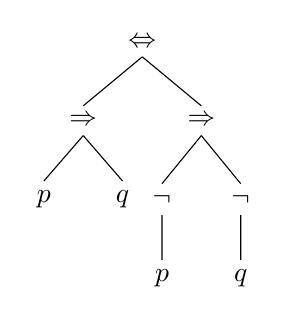
\begin{tikzpicture}[
      level distance=1cm,
      sibling distance=1.5cm,
      level 2/.style={sibling distance=1cm},
      edge from parent path={(\tikzparentnode.south) -- (\tikzchildnode.north)}
    ]
    \node {$\Leftrightarrow$}
      child { 
        node {$\Rightarrow$}
        child { node {$p$} }
        child { node {$q$} }
      }
      child { 
        node {$\Rightarrow$}
        child { node {$\neg$} child { node {$p$} } }
        child { node {$\neg$} child { node {$q$} } }
      };
    \end{tikzpicture}
    }  
  \hfill
  \resizebox{0.35\textwidth}{!}{
    \begin{tikzpicture}[
      level distance=1cm,
      sibling distance=1.5cm,
      level 2/.style={sibling distance=1cm},
      level 3/.style={sibling distance=0.7cm},
      edge from parent path={(\tikzparentnode.south) -- (\tikzchildnode.north)}
    ]
    \node {$\Rightarrow$}
      child { node {$p$} }
      child { 
        node {$\Leftrightarrow$}
        child { node {$q$} }
        child { 
          node {$\neg$}
          child { 
            node {$\Rightarrow$}
            child { node {$p$} }
            child { node {$\neg$} child { node {$q$} } }
          }
        }
      };
    \end{tikzpicture}
    }
  \end{latin}
  \renewcommand{\thefigure}{\lr{2.1}}
  \caption{دو فرمول}
  \end{figure}
  \begin{latin}
  \begin{verbatim}
  Inorder(F):
      if F is a leaf:
          print its label
          return
      Let F1 and F2 be the left and right subtrees of F
      Inorder(F1)
      print the label of the root of F
      Inorder(F2)
  \end{verbatim}
  \end{latin}
  اگر ریشه‌ی $F$ با نماد $\neg$ برچسب‌گذاری شده باشد، زیر‌درخت چپ نادیده گرفته می‌شود و مرحله‌ی \lr{Inorder(F1)} انجام نمی‌گیرد.
  \begin{definition}[تعریف \lr{2.5}]
  اصطلاح «فرمول» برای رشته نیز به‌کار می‌رود، با این فرض که به درخت زیربنایی آن اشاره دارد.
  \end{definition}
  \begin{example}[مثال \lr{2.6}]
  فرمول سمت چپ در شکل \lr{2.1} را در نظر بگیرید. پیمایش درون‌گرد این فرمول به‌صورت زیر است: ابتدا برگ سمت چپ با برچسب $p$ نوشته می‌شود، سپس ریشه‌ی آن که با $\rightarrow$ برچسب‌گذاری شده، سپس برگ سمت راست آن که $q$ است، و سپس ریشه‌ی کل درخت که با $\leftrightarrow$ برچسب‌گذاری شده، و به همین ترتیب ادامه می‌یابد. نتیجه‌ی پیمایش رشته‌ی زیر است:
  \[
  p \rightarrow q \leftrightarrow \neg p \rightarrow \neg q
  \]
  اکنون فرمول سمت راست در شکل \lr{2.1} را در نظر بگیرید. پیمایش آن نیز دقیقاً همین رشته را تولید می‌کند:
  \[
  p \rightarrow q \leftrightarrow \neg p \rightarrow \neg q
  \]
  \end{example}
\subsection*{\lr{2.1.3} رفع ابهام در نمایش رشته‌ای}
   \subsubsection*{پرانتزها}
      
     ساده‌ترین روش برای جلوگیری از ابهام، استفاده از پرانتزها برای حفظ ساختار درخت هنگام تولید رشته است.
      
     \paragraph{الگوریتم \lr{2.7} (نمایش فرمول به‌صورت رشته با پرانتز)} \hfill \\
     \textbf{ورودی:} یک فرمول $A$ از منطق گزاره‌ای \\
     \textbf{خروجی:} نمایش رشته‌ای از $A$ با استفاده از پرانتزها
      
     رویه‌ی بازگشتی زیر را فراخوانی کن: \lr{Inorder(A)}
      
     \begin{latin}
      \begin{verbatim}
      Inorder(F):
          if F is a leaf:
              print its label
              return
          Let F1 and F2 be the left and right subtrees of F
          print '('
          Inorder(F1)
          print the label of the root of F
          Inorder(F2)
          print ')'
      \end{verbatim}
     \end{latin}
   
     اگر ریشه‌ی $F$ با نماد $\neg$ برچسب‌گذاری شده باشد، زیر‌درخت چپ نادیده گرفته می‌شود و مرحله‌ی \lr{Inorder(F1)} انجام نمی‌گیرد.
   
     در این حالت، دو فرمول موجود در شکل \lr{2.1} به دو رشته‌ی متفاوت نگاشته می‌شوند و دیگر ابهامی وجود ندارد:
     \[
     ((p \rightarrow q) \leftrightarrow ((\neg q) \rightarrow (\neg p)))
     \]
     \[
     (p \rightarrow (q \leftrightarrow (\neg (p \rightarrow (\neg q)))))
     \]
   
     مشکل استفاده از پرانتزها آن است که فرمول‌ها را طولانی کرده و خواندن و نوشتن آن‌ها را دشوار می‌سازد.
   
   \subsubsection*{اولویت}
     
     روش دوم برای رفع ابهام در فرمول‌های مبهم، تعریف \textbf{اولویت} (precedence) و \\ \textbf{جهت انجمنی} (associativity) بین عملگرها است، همان‌طور که در حساب معمول انجام می‌شود. برای مثال، عبارت \\ \lr{a * b * c + d * e} بلافاصله به‌صورت \[
     (((a * b) * c) + (d * e))
     \] تفسیر می‌شود.
     
     در مورد فرمول‌های منطقی، ترتیب اولویت از بالا به پایین به‌صورت زیر است:
     
     \[ \\
     \neg \\
     \]
     \[
     \land, \uparrow \\
     \]
     \[
     \lor, \downarrow \\
     \]
     \[
     \rightarrow \\
     \]
     \[
     \leftrightarrow, \oplus
     \]
     عملگرها به‌طور پیش‌فرض \textbf{از راست به چپ} گروه‌بندی می‌شوند (جهت انجاسی راست‌گرا)، یعنی فرمول $a \lor b \lor c$ به‌صورت $a \lor (b \lor c)$ تفسیر می‌شود.
     
     پرانتزها تنها زمانی استفاده می‌شوند که بخواهیم ترتیبی متفاوت از قواعد اولویت و جهت پیش‌فرض را نشان دهیم؛ مانند حساب معمول که در آن \lr{a * (b + c)} به معنای انجام جمع پیش از ضرب است.
     
     با حداقل استفاده از پرانتز، دو فرمول مثال در شکل \lr{2.1} را می‌توان به‌صورت زیر نوشت:
     
     \[
     p \rightarrow q \leftrightarrow \neg q \rightarrow \neg p
     \]
     \[
     p \rightarrow (q \leftrightarrow \neg (p \rightarrow \neg q))
     \]
     
     برای وضوح بیشتر، همیشه می‌توان از پرانتزهای اضافی استفاده کرد؛ مثلاً:
     \[
     (p \lor q) \land (q \lor r)
     \]
     
     عملگرهای بولی $\land$, $\lor$, $\leftrightarrow$, $\oplus$ انجاسی هستند، بنابراین در فرمول‌هایی که شامل تکرار این عملگرها هستند، اغلب پرانتزها حذف می‌شوند؛ مثلاً:
     \[
     p \lor q \lor r \lor s
     \]
     
     اما توجه داشته باشید که عملگرهای $\rightarrow$, $\downarrow$, $\uparrow$ \textbf{غیرانجاسی} هستند، بنابراین استفاده از پرانتز برای جلوگیری از ابهام الزامی است.
     
     اگرچه فرض بر این است که $\rightarrow$ راست‌گرا است و فرمول $p \rightarrow q \rightarrow r$ را به‌صورت $p \rightarrow (q \rightarrow r)$ تفسیر می‌کنیم، اما معمولاً برای وضوح بیشتر، آن را همراه با پرانتز می‌نویسیم:
     \[
     (p \rightarrow q) \rightarrow r
     \]
     
   \subsubsection*{نمادگذاری لهستانی \lr{(Polish Notation)}}
 
    اگر نمایش رشته‌ای یک فرمول با استفاده از پیمایش \textbf{پیش‌گرد} \lr{(preorder traversal)} درخت آن انجام شود، دیگر ابهامی نخواهیم داشت.
 
    \paragraph{الگوریتم \lr{2.8} (نمایش فرمول به‌صورت رشته در نماد لهستانی)} \hfill \\
    \textbf{ورودی:} یک فرمول $A$ از منطق گزاره‌ای \\
    \textbf{خروجی:} نمایش رشته‌ای از $A$ در نمادگذاری لهستانی
 
    رویه‌ی بازگشتی زیر را فراخوانی کن: \lr{Preorder(A)}
 
    \begin{latin}
      \begin{verbatim}
      Preorder(F):
          print the label of the root of F
          if F is a leaf:
              return
          Let F1 and F2 be the left and right subtrees of F
          Preorder(F1)
          Preorder(F2)
      \end{verbatim}
    \end{latin}
 
    اگر ریشه‌ی $F$ با نماد $\neg$ برچسب‌گذاری شده باشد، زیر‌درخت چپ نادیده گرفته می‌شود و مرحله‌ی \lr{Preorder(F1)} انجام نمی‌گیرد.
 
    \begin{example}[مثال \lr{2.9}] رشته‌های مربوط به دو فرمول موجود در شکل \lr{2.1} در نمادگذاری لهستانی به‌صورت زیر هستند:
      \[
      \leftrightarrow\ \rightarrow\ p\ q\ \rightarrow\ \neg p\ \neg q
      \]
      \[
      \rightarrow\ p\ \leftrightarrow\ q\ \neg\ \rightarrow\ p\ \neg q
      \]
    و اکنون دیگر هیچ ابهامی وجود ندارد.
    \end{example}
    فرمول‌هایی که به این صورت نمایش داده می‌شوند، گفته می‌شود در \textbf{نمادگذاری لهستانی} هستند، که به افتخار گروهی از منطق‌دانان لهستانی به رهبری \lr{Jan Łukasiewicz} نام‌گذاری شده است.
 
    ما نمایش درون‌گرد (\lr{infix}) را خواناتر می‌دانیم، چراکه در حساب معمول نیز رایج است. بنابراین نمادگذاری لهستانی معمولاً تنها برای نمایش درونی عبارات حسابی و منطقی در رایانه‌ها استفاده می‌شود. مزیت اصلی آن این است که می‌توان فرمول را در همان ترتیبی که نمادها ظاهر می‌شوند با استفاده از یک \lr{stack} ارزیابی کرد.
 
    اگر فرمول اول را به‌صورت معکوس بازنویسی کنیم (که به آن \textbf{نمادگذاری لهستانی معکوس} یا \lr{RPN} نیز گفته می‌شود):
 
    \[
    q\ \neg\ p\ \neg\ \rightarrow\ q\ p\ \rightarrow\ \leftrightarrow
    \]
 
    می‌توان آن را مستقیماً به دنباله‌ای از دستورات اسمبلی زیر ترجمه کرد:
 
    \begin{latin}
      \begin{verbatim}
      Push q
      Negate
      Push p
      Negate
      Imply
      Push q
      Push p
      Imply
      Equiv
      \end{verbatim}
    \end{latin}
 
    در این روش، عملگرها روی عملوندهایی که در بالای پشته قرار دارند اعمال می‌شوند، سپس عملوندها از پشته خارج (pop) شده و نتیجه روی پشته قرار داده می‌شود.
\subsection*{\lr{2.1.4} \quad استقرا ساختاری}
 
  اگر یک عبارت حسابی مانند \lr{a * b + b * c} را در نظر بگیریم، به‌راحتی می‌توان دید که این عبارت از دو جمله تشکیل شده که با عملگر جمع ترکیب شده‌اند، و هر جمله‌ی جمعی نیز از دو عامل ضرب تشکیل شده است. به‌طور مشابه، هر فرمول گزاره‌ای را می‌توان بر اساس عملگر سطح بالای آن طبقه‌بندی کرد.
 
  \begin{definition}[تعریف \lr{2.10}]
    اگر $A \in \mathscr{F}$ و $A$ یک اتم نباشد، عملگری که ریشه‌ی درخت فرمول $A$ را برچسب‌گذاری می‌کند، \textbf{عملگر اصلی} (\lr{principal operator}) فرمول $A$ نامیده می‌شود.
  \end{definition}
  \begin{example}[مثال \lr{2.11}]
    عملگر اصلی فرمول سمت چپ در شکل \lr{2.1}، عملگر $\leftrightarrow$ و در فرمول سمت راست، عملگر $\rightarrow$ است.\\
  \end{example}

  استقرا ساختاری روشی برای اثبات این است که یک خاصیت برای همه‌ی فرمول‌ها برقرار است. این شکل از استقرا، مشابه \textbf{استقرای عددی} آشنایی است که برای اثبات خاصیت برای همه‌ی اعداد طبیعی به‌کار می‌رود (بخش \lr{A.6} را ببینید). در استقرای عددی:

  \begin{itemize}
    \item \textbf{گام پایه:} اثبات خاصیت برای صفر است، و
    \item \textbf{گام استقرا:} فرض می‌کنیم خاصیت برای عدد دلخواه $n$ برقرار است و سپس اثبات می‌کنیم که برای $n+1$ نیز برقرار خواهد بود.
  \end{itemize}

  بر اساس تعریف \lr{2.10}، یک فرمول یا:
  \begin{itemize}
    \item یک برگ با برچسب اتم است،
    \item یا یک درخت با عملگر اصلی و یک یا دو زیر‌درخت.
  \end{itemize}

  بنابراین، در استقرا ساختاری:
  \begin{itemize}
    \item \textbf{گام پایه:} اثبات خاصیت برای برگ‌ها (اتم‌ها) است.
    \item \textbf{گام استقرا:} اثبات خاصیت برای فرمولی است که از به‌کارگیری عملگر اصلی روی زیر‌فرمول‌ها به‌دست آمده، مشروط بر آنکه خاصیت برای آن زیر‌فرمول‌ها برقرار باشد.
  \end{itemize}

  \begin{theorem}[قضیه \lr{2.12} (استقرا ساختاری). ]
   برای اینکه نشان دهیم خاصیتی برای همه‌ی فرمول‌ها $A \in \mathscr{F}$ برقرار است، کافی است:
   
   \begin{enumerate}
     \item اثبات کنیم که خاصیت برای تمام اتم‌ها $p$ برقرار است.
     \item فرض کنیم خاصیت برای فرمولی مانند $A$ برقرار است و اثبات کنیم که خاصیت برای $\neg A$ نیز برقرار است.
     \item فرض کنیم خاصیت برای فرمول‌های $A_1$ و $A_2$ برقرار است، و اثبات کنیم که خاصیت برای $A_1 \mathbin{\operatorname{op}} A_2$ نیز برقرار است، برای هر یک از عملگرهای دوجمله‌ای.
   \end{enumerate}
  \end{theorem}

  \begin{proof}[اثبات. ]
    فرض کنیم $A$ یک فرمول دلخواه باشد و فرض کنیم که بندهای (۱)، (۲)، (۳) برای خاصیت مورد نظر اثبات شده‌اند. ما نشان می‌دهیم که خاصیت برای $A$ برقرار است، با استفاده از استقرای عددی بر حسب $n$، که ارتفاع درخت مربوط به $A$ است:
    \begin{itemize}
      \item اگر $n = 0$ باشد، درخت یک برگ است، بنابراین $A$ یک اتم $p$ است و خاصیت طبق بند (۱) برقرار است.
      \item اگر $n > 0$ باشد، زیر‌درخت‌های $A$ ارتفاعی برابر با $n - 1$ دارند، بنابراین طبق فرض استقرای عددی، خاصیت برای آن‌ها برقرار است. از آنجا که عملگر اصلی $A$ یا نقیض ($\neg$) است یا یکی از عملگرهای دوجمله‌ای، بنابراین طبق بند (۲) یا (۳)، خاصیت برای $A$ نیز برقرار است.
    \end{itemize}
  \end{proof}
  بعداً نشان خواهیم داد که تمام عملگرهای دوجمله‌ای را می‌توان با ترکیب نقیض و یکی از دو عملگر $\lor$ یا $\land$ تعریف کرد؛ بنابراین، برای اثبات خاصیت برای همه‌ی فرمول‌ها، کافی است از استقرا ساختاری با حالت پایه و تنها دو گام استقرا استفاده کنیم.
\subsection*{\lr{2.1.5} \quad نمادگذاری}
  متأسفانه، در کتاب‌های مختلف منطق ریاضی، نمادهای مورد استفاده برای عملگرهای بولی یکسان نیستند؛ افزون بر این، در زبان‌های برنامه‌نویسی نیز این عملگرها معمولاً با نمادهایی متفاوت از آنچه در منابع ریاضی دیده می‌شود نمایش داده می‌شوند. جدول زیر، برخی از این نمادهای جایگزین را نشان می‌دهد:
  \begin{center}
    \begin{tabular}{|c|c|c|}
    \hline
    \textbf{عملگر} & \textbf{نمادهای جایگزین} & \textbf{زبان \lr{Java}} \\
    \hline
    $\neg$ & \lr{\textasciitilde} & \lr{!} \\
    \hline
    $\land$ & \lr{\&} & \lr{\&}, \lr{\&\&} \\
    \hline
    $\lor$ &  & \lr{|}, \lr{||} \\
    \hline
    $\rightarrow$ & $\supset$, $\Rightarrow$ & \\
    \hline
    $\leftrightarrow$ & $\equiv$, $\Leftrightarrow$ & \\
    \hline
    $\oplus$ & $\not\equiv$ & \lr{\^{}} \\
    \hline
    $\uparrow$ & \lr{|} &  \\
    \hline
    \end{tabular}
  \end{center}
\subsection*{\lr{2.1.6} \quad دستور زبان صوری برای فرمول ها}
  (این زیر‌بخش مستلزم آشنایی با دستور زبان‌های صوری است.)
  به‌جای تعریف فرمول‌ها به‌صورت درختی، می‌توان آن‌ها را به‌شکل رشته‌هایی تعریف کرد که از یک دستور زبان مستقل از متن (\lr{context-free grammar}) تولید می‌شوند.
  \begin{definition}[تعریف \lr{2.13}]
    فرمول‌های منطق گزاره‌ای از دستور زبانی مستقل از متن تولید می‌شوند که نمادهای پایانی (\lr{terminal symbols}) آن به‌صورت زیر تعریف شده‌اند:
    \begin{itemize}
      \item مجموعه‌ای نامتناهی از نمادها به‌نام گزاره‌های اتمی \lr{$\mathcal{P}$}
      \item عملگرهای بولی مطابق با تعریف \lr{2.1}
    \end{itemize}
    قواعد تولید (\lr{production rules}) این دستور زبان به‌صورت زیر هستند:
    \begin{align*}
      \text{fml} &::= p \qquad \text{برای هر } p \in \mathcal{P} \\
      \text{fml} &::= \neg \text{ fml} \\
      \text{fml} &::= \text{fml op fml} \\
      \text{op} &::= \lor \mid \land \mid \rightarrow \mid \leftrightarrow \mid \oplus \mid \uparrow \mid \downarrow
    \end{align*}
    یک فرمول، رشته‌ای است که می‌توان آن را از نماد غیرپایانی \lr{fml} استخراج کرد. مجموعه‌ی تمام فرمول‌هایی که از این دستور زبان به‌دست می‌آیند با نماد $\mathscr{F}$ نمایش داده می‌شود.
    فرآیند تولید (اشتقاق) رشته‌ها در یک دستور زبان صوری را می‌توان با درخت‌های اشتقاق \\ (\lr{derivation trees}) نمایش داد . رشته‌ی نهایی را می‌توان از طریق خواندن برگ‌ها از چپ به راست به‌دست آورد.
  \end{definition}
  \begin{example}[مثال \lr{2.14}]
    در ادامه، فرآیند اشتقاق فرمول زیر در منطق گزاره‌ای نشان داده شده است:
    \[
    p \rightarrow q \leftrightarrow \neg p \rightarrow \neg q
    \]
    \begin{figure}[ht]
    \centering
    \begin{latin}
    \resizebox{0.7\textwidth}{!}{%
    \begin{tikzpicture}[
      level distance=1.5cm,
      sibling distance=4cm,
      level 2/.style={sibling distance=2cm},
      level 3/.style={sibling distance=1cm},
      edge from parent path={(\tikzparentnode.south) -- (\tikzchildnode.north)}
    ]
    \node {fml}
      child { 
        node {fml}
        child { 
        	node {fml}
        	child {node {$p$}}
        }
        child {
        	node {op}
        	child {node {$\Rightarrow$}}
        }
        child { 
        	node {fml} 
        	child {node {$q$}}
        }
      }
      child { 
        node {op}
        child {node {$\Leftrightarrow$}}
        child { 
          node {fml}
          child { 
            node {fml}
            child {node {$\neg$}}
            child {node {fml}
              child {node {$p$}}
            }
          }
          child {
            node {op}
            child {node {$\Rightarrow$}}
          }
          child { 
            node {fml}
            child {node {$\neg$}}
            child {node {fml}
              child {node {$q$}}
            }
          }
        }
      };
    \end{tikzpicture}
    }
    \end{latin}
    \renewcommand{\thefigure}{\lr{2.2}}
    \caption{اشتقاق درخت برای $p \rightarrow q \leftrightarrow \neg p \rightarrow \neg q$ }
    \end{figure}
    درخت مربوطه در شکل \lr{2.2} آمده است. گام‌های اشتقاق به‌صورت زیر هستند:
    \begin{align*}
      1.\quad & \text{fml} \\
      2.\quad & \text{fml op fml} \\
      3.\quad & \text{fml} \leftrightarrow \text{fml} \\
      4.\quad & \text{fml} \rightarrow \text{fml} \leftrightarrow \text{fml} \\
      5.\quad & p \rightarrow \text{fml} \leftrightarrow \text{fml} \\
      6.\quad & p \rightarrow q \leftrightarrow \text{fml} \\
      7.\quad & p \rightarrow q \leftrightarrow \text{fml} \rightarrow \text{fml} \\
      8.\quad & p \rightarrow q \leftrightarrow \neg \text{fml} \rightarrow \text{fml} \\
      9.\quad & p \rightarrow q \leftrightarrow \neg p \rightarrow \text{fml} \\
      10.\quad & p \rightarrow q \leftrightarrow \neg p \rightarrow \neg \text{fml} \\
      11.\quad & p \rightarrow q \leftrightarrow \neg p \rightarrow \neg q
    \end{align*}
  \end{example}
  روش‌هایی که در بخش \lr{2.1.2} برای رفع ابهام معرفی شدند، در اینجا نیز قابل‌استفاده هستند.
  همچنین می‌توان دستور زبان را طوری بازنویسی کرد که پرانتزها را به‌صورت درونی دربر گیرد:
  \begin{align*}
    \text{fml} &::= (\neg \text{fml}) \\
    \text{fml} &::= (\text{fml op fml})
  \end{align*}
  و سپس با تعریف قواعد اولویت، می‌توان تعداد پرانتزها را کاهش داد.
  
  \begin{figure}[ht]
  \centering
    \begin{RTL}
      \begin{tabbing}
      \hspace{6.5cm} \= \kill
        $v_{\mathscr{I}}(A) = \mathscr{I}_A(A)$ \> اگر $A$ یک اتم باشد \\
        $v_{\mathscr{I}}(\neg A) = T$ \> اگر $v_{\mathscr{I}}(A) = F$ \\
        $v_{\mathscr{I}}(\neg A) = F$ \> اگر $v_{\mathscr{I}}(A) = T$ \\
        $v_{\mathscr{I}}(A_1 \lor A_2) = F$ \> اگر $v_{\mathscr{I}}(A_1) = F$ و $v_{\mathscr{I}}(A_2) = F$ \\
        $v_{\mathscr{I}}(A_1 \lor A_2) = T$ \> در غیر این صورت \\
        $v_{\mathscr{I}}(A_1 \land A_2) = T$ \> اگر $v_{\mathscr{I}}(A_1) = T$ و $v_{\mathscr{I}}(A_2) = T$ \\
        $v_{\mathscr{I}}(A_1 \land A_2) = F$ \> در غیر این صورت \\
        $v_{\mathscr{I}}(A_1 \rightarrow A_2) = F$ \> اگر $v_{\mathscr{I}}(A_1) = T$ و $v_{\mathscr{I}}(A_2) = F$ \\
        $v_{\mathscr{I}}(A_1 \rightarrow A_2) = T$ \> در غیر این صورت \\
        $v_{\mathscr{I}}(A_1 \uparrow A_2) = F$ \> اگر $v_{\mathscr{I}}(A_1) = T$ و $v_{\mathscr{I}}(A_2) = T$ \\
        $v_{\mathscr{I}}(A_1 \uparrow A_2) = T$ \> در غیر این صورت \\
        $v_{\mathscr{I}}(A_1 \downarrow A_2) = T$ \> اگر $v_{\mathscr{I}}(A_1) = F$ و $v_{\mathscr{I}}(A_2) = F$ \\
        $v_{\mathscr{I}}(A_1 \downarrow A_2) = F$ \> در غیر این صورت \\
        $v_{\mathscr{I}}(A_1 \leftrightarrow A_2) = T$ \> اگر $v_{\mathscr{I}}(A_1) = v_{\mathscr{I}}(A_2)$ \\
        $v_{\mathscr{I}}(A_1 \leftrightarrow A_2) = F$ \> اگر $v_{\mathscr{I}}(A_1) \ne v_{\mathscr{I}}(A_2)$ \\
        $v_{\mathscr{I}}(A_1 \oplus A_2) = T$ \> اگر $v_{\mathscr{I}}(A_1) \ne v_{\mathscr{I}}(A_2)$ \\
        $v_{\mathscr{I}}(A_1 \oplus A_2) = F$ \> اگر $v_{\mathscr{I}}(A_1) = v_{\mathscr{I}}(A_2)$ \\
      \end{tabbing}
    \end{RTL}
    \renewcommand{\thefigure}{\lr{2.3}}
    \caption{مقادیر منطقی فرمول‌ها}
  \end{figure}
\section*{\lr{2.2} تعبیرها}

  اکنون معناشناسی—یعنی معنای فرمول‌ها—را تعریف می‌کنیم. دوباره به عبارت‌های حسابی فکر کنید. فرض کنید عبارت
  \[
  E\;=\;a * b + 2
  \]
  باشد؛ می‌توانیم برای $a$ و $b$ مقادیری اختصاص دهیم و سپس مقدار عبارت را محاسبه کنیم. مثلاً اگر $a=2$ و $b=3$ باشد، آنگاه مقدار $E$ برابر $8$ خواهد بود. در منطق گزاره‌ای، مقادیر صدق به اتم‌های یک فرمول نسبت داده می‌شوند تا مقدار صدق کل فرمول تعیین شود.

\subsection*{\lr{2.2.1} تعریف یک تعبیر}
  \begin{definition}[تعریف \lr{2.15}]
    فرض کنید $A\in \mathscr{F}$ یک فرمول باشد و $\mathscr{P}_{A}$ مجموعهٔ اتم‌های ظاهرشده در $A$ باشد.  
    یک تعبیر برای $A$، تابع کلی  
    \[
    \mathscr{I}_{A} : \mathscr{P}_{A} \;\longrightarrow\; \{T, F\}
    \]
    است که به هر اتم در $\mathscr{P}_{A}$ یکی از مقادیر صدق $T$ (درست) یا $F$ (نادرست) اختصاص می‌دهد.
  \end{definition}
  \begin{definition}[تعریف \lr{2.16}]
    اگر $\mathscr{I}_{A}$ یک تعبیر برای $A\in \mathscr{F}$ باشد، مقدار صدق $A$ تحت $\mathscr{I}_{A}$، که با
    \[
    v_{\mathscr{I}_{A}}(A)
    \]
    نشان داده می‌شود، به صورت بازگشتی بر اساس ساختار $A$ و مطابق شکل ۲.۳ تعریف می‌شود.
    در عمل، وقتی زمینه مشخص باشد، از خلاصهٔ $\mathscr{I}$ به جای $\mathscr{I}_{A}$ استفاده می‌کنیم و مقدار صدق را به صورت $v_{\mathscr{I}}(A)$ می‌نویسیم.
  \end{definition}
  \begin{example}[مثال \lr{2.17}]
    فرض کنید
    \[
    A \;=\; (p \rightarrow q) \;\leftrightarrow\; (\neg q \rightarrow \neg p)
    \]
    و تعبیر زیر را برای آن در نظر بگیریم:
    \[
    \mathscr{I}_{A}(p)=F,\quad \mathscr{I}_{A}(q)=T.
    \]
    آنگاه مقدار صدق $A$ تحت $\mathscr{I}$ با استفاده از قواعد ارزیابی (شکل ۲.۳) چنین خواهد بود:
    \begin{align*}
    v_{\mathscr{I}}(p) &= \mathscr{I}_{A}(p) = F,\\
    v_{\mathscr{I}}(q) &= \mathscr{I}_{A}(q) = T,\\
    v_{\mathscr{I}}(p\rightarrow q) &= T,\\
    v_{\mathscr{I}}(\neg q) &= F,\\
    v_{\mathscr{I}}(\neg p) &= T,\\
    v_{\mathscr{I}}(\neg q \rightarrow \neg p) &= T,\\
    v_{\mathscr{I}}\bigl((p\rightarrow q)\leftrightarrow(\neg q\rightarrow \neg p)\bigr) &= T.
    \end{align*}
  \end{example}
  \subsection*{تعبیرهای جزئی}
    \begin{definition}[تعریف \lr{2.18}]
      فرض کنید $A\in \mathscr{F}$ یک فرمول در منطق گزاره‌ای باشد و $\mathscr{P}_{A}$ مجموعهٔ اتم‌های ظاهرشده در $A$ باشد.  
      یک «تعبیر جزئی» برای $A$، تابع جزئی  
      \[
      \mathscr{I}_{A} : \mathscr{P}_{A} \rightharpoonup \{T, F\}
      \]
      است که به برخی (نه لزوماً همه)ٔ اتم‌های $\mathscr{P}_{A}$ ارزش $T$ یا $F$ تخصیص می‌دهد.
      ممکن است در یک تعبیر جزئی، بدون این‌که به همهٔ اتم‌ها مقدار داده باشیم، بتوان ارزش صدق فرمول $A$ را مشخص کرد.
    \end{definition}
    \begin{example}[مثال \lr{2.19}]
      فرمول
      \[
      A = p \land q
      \]
      را در نظر بگیرید. یک تعبیر جزئی را در نظر بگیرید که تنها به $p$ مقدار $F$ می‌دهد. روشن است که در این تعبیر جزئی، ارزش صدق $A$ برابر $F$ خواهد بود، زیرا $p \land q$ تنها زمانی $T$ است که هر دو $p$ و $q$ برابر $T$ باشند.
      اگر همین تعبیر جزئی به $p$ مقدار $T$ می‌داد ولی به $q$ مقداری تخصیص نمی‌داد، آنگاه ارزش صدق $A$ قابل تعیین نبود.
    \end{example}
\subsection*{\lr{2.2.2} جداول ارزش}
    \begin{definition}[تعریف \lr{2.20}]
      فرض کنید $A\in \mathscr{F}$ و مجموعهٔ اتم‌های ظاهرشده در $A$، $\mathscr{P}_{A}$، شامل $n$ اتم باشد.  
      یک «جدول ارزش» برای $A$ جدولی است با $n+1$ ستون و $2^{n}$ سطر.  
      ستون‌های اول (تعداد $n$) هر یک یک اتم از $\mathscr{P}_{A}$ را نشان می‌دهند و تمام ترکیب‌های ممکنِ انتساب $T$ یا $F$ به آن‌ها را فهرست می‌کنند (هر سطر یک تعبیر $\mathscr{I}$ را مشخص می‌کند).  
      ستون آخر، ارزش صدق $A$، یعنی $v_{\mathscr{I}}(A)$، را در هر تعبیر $\mathscr{I}$ نمایش می‌دهد.
    \end{definition}
    \begin{example}[مثال \lr{2.21}]
      جدول ارزش فرمول
      \[
      p \;\rightarrow\; q
      \]
      به صورت زیر است:
      \[
      \begin{array}{c c c}
      p & q & p \!\rightarrow\! q\\
      \hline
      T & T & T\\
      T & F & F\\
      F & T & T\\
      F & F & T
      \end{array}
      \]
    \end{example}
    \begin{example}[مثال \lr{2.22}]
      برای فرمول
      \[
      (p\rightarrow q)\;\leftrightarrow\;(\neg q\rightarrow\neg p)
      \]
      ستون‌های میانی ارزش زیرفرمول‌ها را نیز نمایش می‌دهیم:
      \[
      \begin{array}{c c c c c c c}
      p & q & p\!\rightarrow\!q & \neg p & \neg q & \neg q\!\rightarrow\!\neg p & (p\!\rightarrow\!q)\!\leftrightarrow\!(\neg q\!\rightarrow\!\neg p)\\
      \hline
      T & T & T & F & F & T & T\\
      T & F & F & F & T & F & T\\
      F & T & T & T & F & T & T\\
      F & F & T & T & T & T & T
      \end{array}
      \]
    \end{example}
    \begin{example}[مثال \lr{2.23}]
      برای تعبیر \(\mathscr{I}\) با \(\mathscr{I}(p)=T\) و \(\mathscr{I}(q)=F\)، مراحل گام‌به‌گام محاسبهٔ ارزش صدق
      \[
      (p\to q)\;\leftrightarrow\;(\neg q\to\neg p)
      \]
      را می‌توان به صورت زیر در یک جدول نمایش داد. در هر سطر یک مقدار جدید از زیرفرمول اضافه می‌شود:
      
      \[
      \begin{array}{c c c c c c c c c}
      (p & \rightarrow & q) & \leftrightarrow & (\neg & q & \rightarrow & \neg & p)\\
      \hline
      T &   & F &     &     & F   &    &  T  \\
      T &   & F &     &     & F   &    &  T  \\
      T &   & F &     & F   & F   & F  &  T  \\
      T &   & F &     & F   & F   & F  &  T  \\
      T & F & F &     & F   & F   & F  &  T  \\
      T & F & F & T   & F   & F   & F  &  T  \\
      \end{array}
      \]
      اگر همهٔ زیرفرمول‌ها یک‌جا در یک سطر قرار گیرند، همان جدول کامل مثال \lr{2.22} حاصل می‌شود:
      \[
      \begin{array}{c c c c c c c}
      p & q & p\!\to\!q & \neg p & \neg q & \neg q\!\to\!\neg p & (p\!\to\!q)\!\leftrightarrow\!(\neg q\!\to\!\neg p)\\
      \hline
      T & T & T & F & F & T & T\\
      T & F & F & F & T & F & T\\
      F & T & T & T & F & T & T\\
      F & F & T & T & T & T & T
      \end{array}
      \]
    \end{example}
\subsection*{\lr{2.2.3} فهم عملگرهای بولی}
      خوانش طبیعی از عملگرهای بولی «نقیض» ($\neg$) و «و» ($\land$) با معناهای رسمی‌ای که در شکل \lr{۲.۳} تعریف شدند، منطبق است. عملگرهای «ناند» ($\uparrow$) و «نُر» ($\downarrow$) صرفاً نقیض‌های $\land$ و $\lor$ هستند. در این‌جا دربارهٔ عملگرهای «یا» ($\lor$)، «یاِحصری» ($\oplus$) و «التزام» ($\rightarrow$) که معناهای رسمی‌شان می‌تواند موجب سردرگمی شود، توضیح می‌دهیم.
      \subsubsection*{«یا»ی شمولی در برابر «یاِحصری»}
        عملگر «یا» ($\lor$) همان یاِ شمولی است و با «یاِحصری» ($\oplus$) متفاوت است. برای مثال، فرض کنید می‌گوییم:
        \begin{quote}
        ساعت هشت «به سینما می‌روم» یا «به تئاتر می‌روم».
        \end{quote}
        منظور از این گزاره عبارت است از «سینما» $\oplus$ «تئاتر»، چرا که در یک لحظه نمی‌توان هم‌زمان در هر دو مکان بود. این در حالی است که عملگر $\lor$ زمانی مقدار درستی (T) می‌گیرد که دست‌کم یکی از جملات صادق باشد:
        \begin{quote}
        از پاپ‌کورن یا از آب‌نبات می‌خواهید؟
        \end{quote}
        در این حالت می‌توان گفت: «پاپ‌کورن» $\lor$ «آب‌نبات»، زیرا ممکن است هم پاپ‌کورن و هم آب‌نبات را بخواهیم.  
        برای $\lor$ کافی است یکی از زیرجملات صادق باشد تا کلِ عبارت صادق شود؛ بنابراین عبارت نامأنوس زیر نیز صادق است، تنها به این دلیل که جملهٔ اول به تنهایی کافی است:
        \[
        \text{«زمین دورتر از خورشید است تا ونوس»} \lor \text{«$1+1=3$»}
        \]
      \paragraph{تفاوت وقتی هر دو زیرجمله صادق باشند}
        \begin{itemize}
          \item با $\lor$: اگر دو زیرجمله صادق باشند، یاِ شمولی همچنان صادق است.
          \item با $\oplus$: اگر دو زیرجمله صادق باشند، یاِحصری نادرست است (چرا که حصری بودن ایجاب می‌کند دقیقاً یکی صادق باشد).
        \end{itemize}
        اینگونه می‌توان تفکیک روشنی میان $\lor$ و $\oplus$ قائل شد.
      \subsubsection*{یا شمولی در برابر یا اختصاصی در زبان‌های برنامه‌نویسی}
      وقتی \lr{or} در زمینهٔ زبان‌های برنامه‌نویسی به کار می‌رود، معمولاً منظور همان یا شمولی است:
        \begin{latin}
        \begin{verbatim}
        if (index < min || index > max) /* There is an error */
        \end{verbatim}
        \end{latin}
        در این مثال، درستی یکی از دو زیرعبارت باعث اجرای دستورات بعدی می‌شود. عملگر \verb| || | در اصل یک عملگر بولی واقعی نیست، زیرا از «ارزیابی کوتاه‌مدت» \lr{(short-circuit evaluation)} استفاده می‌کند: اگر زیرعبارت اول درست باشد، زیرعبارت دوم اصلاً ارزیابی نمی‌شود، چرا که نتیجهٔ آن نمی‌تواند تصمیم به اجرای ادامهٔ دستورات را تغییر دهد.
        برای ارزیابی بولی واقعی می‌توان از عملگر \verb!|! استفاده کرد؛ این عملگر معمولاً هنگام کار با بردارهای بیتی به کار می‌رود:
        \begin{latin}
        \begin{verbatim}
        mask1 = 0xA0;
        mask2 = 0x0A;
        mask  = mask1 | mask2;
        \end{verbatim}
        \end{latin}
        یاِحصری ($\oplus$ در منطق) که در زبان‌های برنامه‌نویسی با نماد \verb|^| نمایش داده می‌شود، برای رمزگذاری و رمزگشایی در سیستم‌های تصحیح خطا و رمزنگاری کاربرد دارد. دلیل این کار این است که با استفادهٔ دوباره از آن می‌توان مقدار اصلی را بازیافت. فرض کنید داده‌ای را با یک کلید مخفی رمزگذاری کنیم:
        \begin{latin}
        \begin{verbatim}
        codedMessage = data ^ key;
        \end{verbatim}
        \end{latin}
        گیرندهٔ پیام نیز می‌تواند به این صورت آن را رمزگشایی نماید:
        \begin{latin}
        \begin{verbatim}
        clearMessage = codedMessage ^ key;
        \end{verbatim}
        \end{latin}
        با دقت در محاسبهٔ زیر می‌بینیم که مقدار اولیه بازیابی می‌شود:
        \begin{latin}
        \begin{verbatim}
        clearMessage == codedMessage ^ key
                     == (data ^ key) ^ key
                     == data ^ (key ^ key)
                     == data ^ false
                     == data
        \end{verbatim}
        \end{latin}
        
      \subsubsection*{التزام (Implication)}
        عملگر $p \rightarrow q$ «التزام مادی» نامیده می‌شود؛ $p$ مقدم و $q$ مؤخر نامیده می‌شود. التزام مادی ادعای علیّت نمی‌کند؛ یعنی نمی‌گوید که مقدم، باعث مؤخر شده یا حتی با آن مرتبط است. یک التزام مادی تنها بیان می‌کند که اگر مقدم درست باشد، مؤخر نیز باید درست باشد؛ بنابراین تنها زمانی که مقدم درست و مؤخر نادرست باشد می‌توان آن را نادرست یافت.
        برای مثال، به دو گزارهٔ زیر توجه کنید:
        \[
        \text{«زمین دورتر از خورشید است تا ونوس»} \rightarrow \text{«$1+1=3$»}
        \]
        این گزاره نادرست است، چرا که مقدم درست و مؤخر نادرست است. اما:
        \[
        \text{«زمین دورتر از خورشید است تا مریخ»} \rightarrow \text{«$1+1=3$»}
        \]
        این گزاره صادق است، زیرا نادرستی مقدم به تنهایی برای صادق بودن کل التزام کافی است.
\subsection*{\lr{2.2.4} تعبیری برای یک مجموعه از فرمول‌ها}
      \begin{definition}[تعریف \lr{2.24}]
        فرض کنید
        \[
        S = \{A_1, A_2, \dots\}
        \]
        مجموعه‌ای از فرمول‌ها باشد و بگذارید
        \[
        \mathscr{P}_S = \bigcup_i \mathscr{P}_{A_i}
        \]
        که $\mathscr{P}_S$ مجموعهٔ تمام اتم‌هایی است که در فرمول‌های $S$ ظاهر می‌شوند.
        
        یک \emph{تعبیر برای $S$} تابعی است به صورت:
        \[
        \mathscr{I}_S : \mathscr{P}_S \to \{T, F\}.
        \]
        
        برای هر $A_i \in S$، مقدار صدق $v_{\mathscr{I}_S}(A_i)$ (یعنی ارزش صدق $A_i$ تحت تعبیر $\mathscr{I}_S$) دقیقاً همانند تعریف \lr{2.16} تعیین می‌شود.
        
        تعریف $\mathscr{P}_S$ به‌صورت اجتماع مجموعه‌های اتم‌ها در فرمول‌های $S$ تضمین می‌کند که به هر اتم دقیقاً یک مقدار «درست» یا «غلط» اختصاص یابد.
      \end{definition}
        
      \begin{example}[مثال \lr{2.25}]
        فرض کنید
        \[
        S = \left\{\, p \rightarrow q,\; p,\; q \land r,\; p \lor s \leftrightarrow s \land q \,\right\}
        \]
        و تعبیر $\mathscr{I}_S$ چنان است که
        \[
        \mathscr{I}_S(p) = T, \quad \mathscr{I}_S(q) = F, \quad \mathscr{I}_S(r) = T, \quad \mathscr{I}_S(s) = T.
        \]
        
        آنگاه مقادیر صدق اعضای $S$ به‌صورت زیر محاسبه می‌شوند:
        \[
        \begin{aligned}
        v_{\mathscr{I}_S}(p \rightarrow q) &= F, \\
        v_{\mathscr{I}_S}(p)               &= \mathscr{I}_S(p) = T, \\
        v_{\mathscr{I}_S}(q \land r)       &= F, \\
        v_{\mathscr{I}_S}(p \lor s)        &= T, \\
        v_{\mathscr{I}_S}(s \land q)       &= F, \\
        v_{\mathscr{I}_S}(p \lor s \leftrightarrow s \land q) &= F.
        \end{aligned}
        \]
      \end{example}
\section*{\lr{2.3} معادل‌های منطقی}
    \begin{definition}[تعریف \lr{2.26}]
      فرض کنید $A_1, A_2 \in \mathscr{F}$. اگر برای همهٔ تعبیرها $\mathscr{I}$ داشته باشیم
      \[
      v_{\mathscr{I}}(A_1) = v_{\mathscr{I}}(A_2),
      \]
      آنگاه می‌گوییم $A_1$ \emph{معادل منطقی} $A_2$ است و با
      \[
      A_1 \equiv A_2
      \]
      نشان می‌دهیم.
    \end{definition}
      
    \begin{example}[مثال \lr{2.27}]
      آیا فرمول
      \[
      p \lor q
      \]
      معادل منطقی
      \[
      q \lor p
      \]
      است؟ چهار تعبیر متمایز برای اتم‌های $p$ و $q$ وجود دارد:
      
      \begin{center}
      \begin{tabular}{|c|c|c|c|}
      \hline
      $\mathscr{I}(p)$ & $\mathscr{I}(q)$ & $v_{\mathscr{I}}(p \lor q)$ & $v_{\mathscr{I}}(q \lor p)$ \\
      \hline
      $T$ & $T$ & $T$ & $T$ \\
      $T$ & $F$ & $T$ & $T$ \\
      $F$ & $T$ & $T$ & $T$ \\
      $F$ & $F$ & $F$ & $F$ \\
      \hline
      \end{tabular}
      \end{center}
      
      چون در همهٔ این تعبیرها صدق دو فرمول یکسان است، داریم:
      \[
      p \lor q \;\equiv\; q \lor p.
      \]
    \end{example}
      
    \begin{theorem}[قضیه \lr{2.28}]
      برای هر $A_1, A_2 \in \mathscr{F}$،
      \[
      A_1 \lor A_2 \;\equiv\; A_2 \lor A_1.
      \]
    \end{theorem}
      
    \begin{proof}
      بگذارید $\mathscr{I}$ یک تعبیر دلخواه برای $A_1 \lor A_2$ باشد. واضح است که $\mathscr{I}$ تعبیر معتبری برای $A_2 \lor A_1$ نیز هست، زیرا:
      \[
      \mathscr{P}_{A_1} \cup \mathscr{P}_{A_2} \;=\; \mathscr{P}_{A_2} \cup \mathscr{P}_{A_1}.
      \]
      
      از آنجا که $\mathscr{P}_{A_1} \subseteq \mathscr{P}_{A_1} \cup \mathscr{P}_{A_2}$، تعبیر $\mathscr{I}$ به همهٔ اتم‌های $A_1$ مقدار می‌دهد و بنابراین تعبیر معتبری برای $A_1$ است؛ به‌طور مشابه برای $A_2$.
      
      اکنون داریم:
      \[
      v_{\mathscr{I}}(A_1 \lor A_2) = T
      \;\Longleftrightarrow\;
      v_{\mathscr{I}}(A_1) = T \;\lor\; v_{\mathscr{I}}(A_2) = T,
      \]
      و
      \[
      v_{\mathscr{I}}(A_2 \lor A_1) = T
      \;\Longleftrightarrow\;
      v_{\mathscr{I}}(A_2) = T \;\lor\; v_{\mathscr{I}}(A_1) = T.
      \]
      
      اگر $v_{\mathscr{I}}(A_1) = T$، آن‌گاه
      \[
      v_{\mathscr{I}}(A_1 \lor A_2) = T = v_{\mathscr{I}}(A_2 \lor A_1),
      \]
      و همین‌طور اگر $v_{\mathscr{I}}(A_2) = T$.
      
      چون $\mathscr{I}$ دلخواه بود، نتیجه می‌گیریم:
      \[
      A_1 \lor A_2 \equiv A_2 \lor A_1.
      \]
    \end{proof}

\subsection*{\lr{2.3.1} \quad (رابطهٔ بین \lr{$\leftrightarrow$} و \lr{$\equiv$})}
    عملگر «معادل» (\lr{$\leftrightarrow$}) یک \emph{عملگر بولی} در منطق گزاره‌ای است و می‌تواند در فرمول‌های این منطق ظاهر شود. اما «معادل منطقی» (\lr{$\equiv$}) یک عملگر بولی نیست؛ بلکه نشانه‌ای برای ویژگی یک جفت فرمول در منطق گزاره‌ای است. این دو مفهوم می‌توانند سردرگمی ایجاد کنند، زیرا ما از واژگان مشابه هم برای زبان مَحْتوایی (در اینجا زبان منطق گزاره‌ای) و هم برای زبان مَدرِکی—آنچه برای استدلال دربارهٔ زبان محتوا استفاده می‌کنیم—بهره می‌بریم.
    
    با این حال، معادل بودن (\lr{$\leftrightarrow$}) و معادل منطقی (\lr{$\equiv$}) ارتباط نزدیکی دارند، چنان‌که در قضیهٔ زیر نشان داده شده است:
    
    \begin{theorem}[قضیه \lr{2.29}]
      $A_1 \equiv A_2$ اگر و تنها اگر $A_1 \leftrightarrow A_2$ در هر تعبیر صدق کند.
    \end{theorem}
    
    \begin{proof}
      فرض کنید $A_1 \equiv A_2$ و $\mathscr{I}$ یک تعبیر دلخواه باشد. از تعریف معادل منطقی می‌دانیم:
      \[
      v_{\mathscr{I}}(A_1) = v_{\mathscr{I}}(A_2).
      \]
      طبق جدول ارزش صدق (شکل \lr{2.3})، در این صورت داریم:
      \[
      v_{\mathscr{I}}(A_1 \leftrightarrow A_2) = T.
      \]
      از آنجا که $\mathscr{I}$ دلخواه بود، نتیجه می‌شود $A_1 \leftrightarrow A_2$ در همهٔ تعبیرها درست است.
      
      اثبات جهت معکوس (یعنی اگر $A_1 \leftrightarrow A_2$ در همهٔ تعبیرها درست باشد، آنگاه $A_1 \equiv A_2$) به‌صورتی مشابه انجام می‌پذیرد.
    \end{proof}
    
    \begin{figure}[ht]
      \centering
      \begin{latin}
      \resizebox{0.7\textwidth}{!}{
      \begin{tikzpicture}[
        level distance=1.5cm,
        sibling distance=4cm,
        level 2/.style={sibling distance=2cm},
        level 3/.style={sibling distance=1cm},
        edge from parent path={(\tikzparentnode.south) -- (\tikzchildnode.north)}
      ]
      \node {$\leftrightarrow$}
        child { 
          node {$\rightarrow$}
          child {node {$p$}}
          child {node {$p$}}
        }
        child { 
          node {$\rightarrow$}
          child {
            node {$\neg$}
            child {node {$p$}}
          }
          child {
            node {$\neg$}
            child {node {$q$}}
          }
        };
      \end{tikzpicture}
      }
      \\
      \resizebox{0.2\textwidth}{!}{
        \begin{tikzpicture}[
          level distance=0.75cm,
          sibling distance=0.75cm,
          level 2/.style={sibling distance=1cm},
          edge from parent path={(\tikzparentnode.south) -- (\tikzchildnode.north)}
        ]
        \node {$\rightarrow$}
          child { 
            child {node {$p$}}
            child {node {$p$}}
          };
        \end{tikzpicture}
      }
      \hfill
      \resizebox{0.1\textwidth}{!}{
        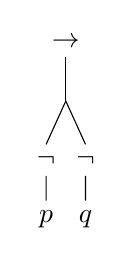
\begin{tikzpicture}[
          level distance=0.75cm,
          sibling distance=0.75cm,
          level 2/.style={sibling distance=0.5cm},
          level 3/.style={sibling distance=0.5cm},
          edge from parent path={(\tikzparentnode.south) -- (\tikzchildnode.north)}
        ]
        \node {$\rightarrow$}
          child { 
            child {
              node {$\neg$}
              child {node {$p$}}
            }
            child {
              node {$\neg$}
              child {node {$q$}}
            }
          };
        \end{tikzpicture}
      }
      \hfill
      \resizebox{0.1\textwidth}{!}{
        \begin{tikzpicture}[
          level distance=0.75cm,
          sibling distance=0.75cm,
          level 2/.style={sibling distance=0.5cm},
          level 3/.style={sibling distance=0.5cm},
          edge from parent path={(\tikzparentnode.south) -- (\tikzchildnode.north)}
        ]
        \node {$\neg$}
          child { 
            child { node {$p$} }
          };
          
        \end{tikzpicture}
      }
      \hfill
      \resizebox{0.1\textwidth}{!}{
        \begin{tikzpicture}[
          level distance=0.75cm,
          sibling distance=0.75cm,
          level 2/.style={sibling distance=0.5cm},
          level 3/.style={sibling distance=0.5cm},
          edge from parent path={(\tikzparentnode.south) -- (\tikzchildnode.north)}
        ]
        \node {$\neg$}
          child { 
            child { node {$q$} }
          };
          
        \end{tikzpicture}
      }
      \hfill
      \resizebox{0.1\textwidth}{!}{
        \begin{tikzpicture}[
          level distance=0.75cm,
          sibling distance=0.75cm,
          level 2/.style={sibling distance=0.5cm},
          level 3/.style={sibling distance=0.5cm},
          edge from parent path={(\tikzparentnode.south) -- (\tikzchildnode.north)}
        ]
        \node {$p$};
          
        \end{tikzpicture}
      }
      \hfill
      \resizebox{0.1\textwidth}{!}{
        \begin{tikzpicture}[
          level distance=0.75cm,
          sibling distance=0.75cm,
          level 2/.style={sibling distance=0.5cm},
          level 3/.style={sibling distance=0.5cm},
          edge from parent path={(\tikzparentnode.south) -- (\tikzchildnode.north)}
        ]
        \node {$q$};
          
        \end{tikzpicture}
      }
      \end{latin}
      \renewcommand{\thefigure}{\lr{2.4}}
      \caption{زیر فرمول ها}
      \end{figure}
\subsection*{\lr{2.3.2} جایگزینی}
      معادل منطقی توجیه‌کنندهٔ جایگزینی یک فرمول به‌جای فرمول دیگری است.
      
      \begin{definition}[تعریف \lr{2.30}]
        اگر $A$ زیردرختی از فرمول $B$ باشد، آنگاه می‌گوییم $A$ یک \emph{زیرفرمول} از $B$ است. اگر $A$ دقیقاً با $B$ یکسان نباشد، آن را \emph{زیرفرمول درست} $B$ می‌نامیم.
      \end{definition}
      
      \begin{example}[مثال \lr{2.31}]
        شکل \lr{2.4} فرمول
        \[
        (p \to q) \;\leftrightarrow\; (\neg p \to \neg q)
        \]
        (فرمول سمت چپ شکل \lr{2.1}) و زیرفرمول‌های درست آن را نشان می‌دهد.
        اگر به‌صورت رشته نمایش داده شود، زیرفرمول‌های درست عبارتند از:
        \[
        p \to q,\quad \neg p \to \neg q,\quad \neg p,\quad \neg q,\quad p,\quad q.
        \]
      \end{example}
      
      \begin{definition}[تعریف \lr{2.32}]
        فرض کنید $A$ یک زیرفرمول از $B$ باشد و $A'$ هر فرمول دلخواهی باشد.
        $B\{A \leftarrow A'\}$ یعنی جایگزینی $A'$ به‌جای $A$ در $B$، فرمولی است که از $B$ به‌دست می‌آید وقتی همهٔ زیردرخت‌های متناظر با $A$ در $B$ با $A'$ جایگزین شوند.
      \end{definition}
      
      \begin{example}[مثال \lr{2.33}]
        بگذارید
        \[
        B = (p \to q) \leftrightarrow (\neg p \to \neg q),\quad
        A = p \to q,\quad
        A' = \neg p \lor q.
        \]
        آنگاه
        \[
        B\{A \leftarrow A'\}
        \;=\;
        (\neg p \lor q) \;\leftrightarrow\; (\neg q \to \neg p).
        \]
      \end{example}
      
      اگر در فرمول $B$، یک زیرفرمول $A$ با فرمولی که معادل منطقی $A$ است جایگزین شود، ارزش‌گذاری $B$ در هیچ تعبیر تغییر نمی‌کند.
      
      \begin{theorem}[قضیه \lr{2.34}]
        فرض کنید $A$ زیرفرمولی از $B$ باشد و $A'$ فرمولی باشد که $A \equiv A'$. آنگاه
        \[
        B \;\equiv\; B\{A \leftarrow A'\}.
        \]
      \end{theorem}
      
      \begin{proof}
        بگذارید $\mathscr{I}$ یک تعبیر دلخواه باشد. چون $A \equiv A'$، پس:
        \[
        v_{\mathscr{I}}(A) = v_{\mathscr{I}}(A').
        \]
        باید نشان دهیم:
        \[
        v_{\mathscr{I}}(B)
        =
        v_{\mathscr{I}}\bigl(B\{A \leftarrow A'\}\bigr).
        \]
        اثبات با استقرا بر عمق $d$ بالاترین وقوع زیردرخت $A$ در $B$ انجام می‌شود:
        
        \begin{itemize}
          \item \textbf{حالت پایه} ($d = 0$):  
            در این حالت، تنها یک وقوع از $A$ وجود دارد که همان خود $B$ است. پس:
            \[
            v_{\mathscr{I}}(B)
            = v_{\mathscr{I}}(A)
            = v_{\mathscr{I}}(A')
            = v_{\mathscr{I}}\bigl(B\{A \leftarrow A'\}\bigr).
            \]
          \item \textbf{گام استقرا} ($d > 0$):  
            در این حالت، $B$ یکی از دو صورت زیر است:
            \begin{enumerate}
              \item $B = \neg B_1$,
              \item $B = B_1\;\mathrm{op}\;B_2$ برای برخی فرمول‌های $B_1, B_2$ و یک عملگر بولی $\mathrm{op}$.
            \end{enumerate}
            در هر دو صورت، عمق $A$ در زیردرخت‌های $B_1$ و $B_2$ کمتر از $d$ است. بنابراین، بر اساس فرض استقرا:
            \[
            v_{\mathscr{I}}(B_1)
            = v_{\mathscr{I}}\bigl(B_1\{A \leftarrow A'\}\bigr),
            \quad
            v_{\mathscr{I}}(B_2)
            = v_{\mathscr{I}}\bigl(B_2\{A \leftarrow A'\}\bigr).
            \]
            پس بر اساس تعریف ارزش‌گذاری برای عملگرهای بولی:
            \[
            v_{\mathscr{I}}(B)
            = v_{\mathscr{I}}\bigl(B\{A \leftarrow A'\}\bigr).
            \]
        \end{itemize}
        در نتیجه، از آنجا که $\mathscr{I}$ دلخواه بود داریم:
        \[
        B \equiv B\{A \leftarrow A'\}.
        \]
      \end{proof}
\subsection*{\lr{2.3.3}  فرمول‌های معادل منطقی}
      جایگزینی فرمول‌های معادل منطقی اغلب انجام می‌شود، برای مثال در ساده‌سازی فرمول‌ها، و آشنایی با معادل‌های پرکاربرد فهرست‌شده در این زیربخش ضروری است. اثبات آن‌ها از تعاریف ابتدایی به‌دست می‌آید و به‌عنوان تمرین باقی گذاشته شده است.
      
      \subsubsection*{جذب ثابت‌ها \lr{(Absorption of Constants)}}
      اجازه دهید نحو فرمول‌های بولی را طوری گسترش دهیم که دو گزارهٔ اتمی ثابت \(\text{true}\) و \(\text{false}\) را نیز شامل شود. (نمادهای دیگر: \(\top\) برای \(\text{true}\) و \(\bot\) برای \(\text{false}\).) معنای آن‌ها به صورت زیر تعریف می‌شود:
      \[
      \mathscr{I}(\text{true}) = T
      \quad\text{و}\quad
      \mathscr{I}(\text{false}) = F
      \]
      برای هر تعبیر \(\mathscr{I}\).  
      این نمادها را نباید با مقادیر صدق \(T\) و \(F\) که در تعریف ارزش‌گذاری به‌کار می‌روند، اشتباه گرفت. همچنین می‌توان \(\text{true}\) و \(\text{false}\) را به‌ترتیب به‌عنوان اختصار برای فرمول‌های زیر در نظر گرفت:
      \[
      p \lor \neg p
      \quad\text{و}\quad
      p \land \neg p.
      \]
      وقوع یک ثابت در فرمول ممکن است آن را چنان فرو بکاهد که عملگر دودویی بی‌نیاز شود یا حتی فرمول به یک ثابت تبدیل شود:
      \[
      \begin{aligned}
      A \lor \text{true} &\equiv \text{true}
      &\quad
      A \land \text{true} &\equiv A\\
      A \lor \text{false} &\equiv A
      &\quad
      A \land \text{false} &\equiv \text{false}\\
      A \to \text{true} &\equiv \text{true}
      &\quad
      \text{true} \to A &\equiv A\\
      A \to \text{false} &\equiv \neg A
      &\quad
      \text{false} \to A &\equiv \text{true}\\
      A \leftrightarrow \text{true} &\equiv A
      &\quad
      A \oplus \text{true} &\equiv \neg A\\
      A \leftrightarrow \text{false} &\equiv \neg A
      &\quad
      A \oplus \text{false} &\equiv A
      \end{aligned}
      \]
      
      \subsubsection*{عملوندهای همسان \lr{(Identical Operands)}}
      فروپاشی (collapse) همچنین وقتی رخ می‌دهد که هر دو عملوند یکسان باشند یا یکی نقیض دیگری:
      \[
      \begin{aligned}
      A &\equiv \neg\neg A,\\
      A &\equiv A \land A
      &\quad
      A &\equiv A \lor A,\\
      A \lor \neg A &\equiv \text{true}
      &\quad
      A \land \neg A &\equiv \text{false},\\
      A \to A &\equiv \text{true},\\
      A \leftrightarrow A &\equiv \text{true}
      &\quad
      A \oplus A &\equiv \text{false},\\
      \neg A &\equiv A \uparrow A
      &\quad
      \neg A &\equiv A \downarrow A.
      \end{aligned}
      \]
      
      \subsubsection*{جابجایی، پیمایش‌پذیری، و توزیع‌پذیری}
      اپراتورهای دودویی بولی—به‌جز «تضمین» (\(\to\))—هم جابجایی‌پذیرند و هم پیمایش‌پذیر:
      \[
      \begin{aligned}
      A \lor B &\equiv B \lor A
      &\quad
      A \land B &\equiv B \land A,\\
      A \leftrightarrow B &\equiv B \leftrightarrow A
      &\quad
      A \oplus B &\equiv B \oplus A,\\
      A \uparrow B &\equiv B \uparrow A
      &\quad
      A \downarrow B &\equiv B \downarrow A.
      \end{aligned}
      \]
      با ورود نقیض، جهت یک تضمین می‌تواند وارونه شود:
      \[
      A \to B \;\equiv\; \neg B \to \neg A.
      \]
      فرمول \(\neg B \to \neg A\) را \emph{مخالف‌مقدم} (contrapositive) \(\,A \to B\) می‌نامند.
      
      جمع‌گزاره (\(\lor\))، ضرب‌گزاره (\(\land\))، معادل (\(\leftrightarrow\)) و نامعادل (\(\oplus\)) پیمایش‌پذیرند:
      \[
      \begin{aligned}
      A \lor (B \lor C) &\equiv (A \lor B) \lor C
      &\quad
      A \land (B \land C) &\equiv (A \land B) \land C,\\
      A \leftrightarrow (B \leftrightarrow C) &\equiv (A \leftrightarrow B) \leftrightarrow C
      &\quad
      A \oplus (B \oplus C) &\equiv (A \oplus B) \oplus C.
      \end{aligned}
      \]
      ولی تضمین (\(\to\))، nor (\(\downarrow\)) و nand (\(\uparrow\)) پیمایش‌پذیر نیستند.
      
      همچنین، جمع‌گزاره و ضرب‌گزاره بر یکدیگر توزیع‌پذیرند:
      \[
      \begin{aligned}
      A \lor (B \land C) &\equiv (A \lor B) \land (A \lor C),\\
      A \land (B \lor C) &\equiv (A \land B) \lor (A \land C).
      \end{aligned}
      \]
      
      \subsubsection*{تعریف یک عملگر به‌واسطهٔ عملگر دیگر}
      در اثبات قضایا با استقرا ساختاری، گام استقرایی باید برای هر عملگر دودویی جداگانه انجام شود. این گام‌ها ساده‌تر می‌شوند اگر بتوان عملگرهای خاص را با جایگزینی زیرفرمول‌هایی حذف کرد و فقط از مجموعه‌ای از عملگرهای پایه بهره گرفت. مثلاً معادل (\(\leftrightarrow\)) را می‌توان با ترکیب تضمین و ضرب‌گزاره تعریف کرد.
      
      همچنین، برخی الگوریتم‌ها برای تبدیل فرمول به شکل نرمال، نیازمند حذف برخی عملگرها هستند. فهرست معادل‌هایی که برای این کار کاربرد دارند:
      \[
      \begin{aligned}
      A \leftrightarrow B &\equiv (A \to B) \land (B \to A)
      &\quad
      A \oplus B &\equiv \neg(A \to B) \lor \neg(B \to A),\\
      A \to B &\equiv \neg A \lor B
      &\quad
      A \to B &\equiv \neg(A \land \neg B),\\
      A \lor B &\equiv \neg(\neg A \land \neg B)
      &\quad
      A \land B &\equiv \neg(\neg A \lor \neg B),\\
      A \lor B &\equiv \neg A \to B
      &\quad
      A \land B &\equiv \neg(A \to \neg B).
      \end{aligned}
      \]
      تعریف ضرب‌گزاره برحسب جمع‌گزاره و نقیض و بالعکس را \emph{قضایای دمورگان} \lr{(De Morgan’s laws)} می‌نامند.
\section*{\lr{2.4} مجموعه‌ای از عملگرهای بولی}

      از دوران ابتدایی مدرسه به ما آموخته‌اند که چهار عملگر پایه در حساب عبارت‌اند از: جمع، تفریق، ضرب و تقسیم. بعدها با عملگرهای اضافی‌تری مانند مدولو (مانده) و قدر مطلق آشنا می‌شویم. از سوی دیگر، از دید نظری می‌دانیم ضرب و تقسیم در حقیقت زائد هستند، زیرا می‌توان آن‌ها را برحسب جمع و تفریق تعریف کرد.
      
      در این بخش، به دو پرسش می‌پردازیم:
      \begin{enumerate}
        \item چه عملگرهای بولی وجود دارند؟
        \item چه مجموعه‌ای از این عملگرها «کافی» است، به این معنا که بتوان همهٔ عملگرهای دیگر را تنها با استفاده از عملگرهای آن مجموعه تعریف کرد؟
      \end{enumerate}

\subsection*{\lr{2.4.1} عملگرهای بولی یگانی و دودویی}
      از آنجایی که تنها دو مقدار بولی $T$ و $F$ وجود دارد، تعداد عملگرهای با $n$ ورودی برابر است با $2^{2^n}$، زیرا برای هر یک از $n$ گزارهٔ ورودی می‌توان یکی از دو مقدار $T$ یا $F$ را انتخاب کرد (در مجموع $2^n$ ترکیب ممکن) و برای هر یک از این ترکیب‌ها می‌توان مقدار خروجی را $T$ یا $F$ قرار داد. در اینجا خود را به عملگرهای تک‌جایی (یک‌جایی) و دو‌جایی (دو‌جایی) محدود می‌کنیم.
      \paragraph{عملگرهای تک‌جایی}
      جدول زیر چهار عملگر تک‌جایی ممکن $\circ_1,\dots,\circ_4$ را نشان می‌دهد. ستون اول مقدار ورودی $x$ را و ستون‌های بعدی مقدار $\circ_n(x)$ را می‌دهند:
      \[
      \begin{array}{c|cccc}
      x & \circ_1 & \circ_2 & \circ_3 & \circ_4\\\hline
      $T$ & $T$ & $T$ & $F$ & $F$\\
      $F$ & $T$ & $F$ & $T$ & $F$
      \end{array}
      \]
      \paragraph{عملگرهای دو‌جایی}
      شکل \lr{2.5} عملگرهای دو‌جایی $\circ_1,\dots,\circ_{16}$ را بر اساس مقادیر ورودی $(x_1,x_2)$ فهرست می‌کند:
      \begin{figure}[ht]
      \centering
      \[
      \begin{array}{cc|cccccccc}
      x_1 & x_2 & \circ_1 & \circ_2 & \circ_3 & \circ_4 & \circ_5 & \circ_6 & \circ_7 & \circ_8\\\hline
      $T$ & $T$ & $T$ & $T$ & $T$ & $T$ & $T$ & $T$ & $T$ & $T$\\
      $T$ & $F$ & $T$ & $T$ & $T$ & $T$ & $F$ & $F$ & $F$ & $F$\\
      $F$ & $T$ & $T$ & $T$ & $F$ & $F$ & $T$ & $T$ & $F$ & $F$\\
      $F$ & $F$ & $T$ & $F$ & $T$ & $F$ & $T$ & $F$ & $T$ & $F$
      \end{array}
      \]
      \[
      \begin{array}{cc|cccccccc}
      x_1 & x_2 & \circ_{9} & \circ_{10} & \circ_{11} & \circ_{12} & \circ_{13} & \circ_{14} & \circ_{15} & \circ_{16}\\\hline
      $T$ & $T$ & $F$ & $F$ & $F$ & $F$ & $F$ & $F$ & $F$ & $F$\\
      $T$ & $F$ & $T$ & $T$ & $T$ & $T$ & $F$ & $F$ & $F$ & $F$\\
      $F$ & $T$ & $T$ & $T$ & $F$ & $F$ & $T$ & $T$ & $F$ & $F$\\
      $F$ & $F$ & $T$ & $F$ & $T$ & $F$ & $T$ & $F$ & $T$ & $F$
      \end{array}
      \]
      \renewcommand{\thefigure}{\lr{2.5}}
      \caption{عملگر های بولی دو جایی}
      \end{figure}
      از چهار عملگر تک‌جایی، سه تای آن‌ها بدیهی هستند: $\circ_1$ و $\circ_4$ عملگرهای ثابتند (همیشه $T$ یا همیشه $F$) و $\circ_2$ عملگر هویت است که ورودی را بدون تغییر برمی‌گرداند. تنها عملگر غیربدیهی تک‌جایی $\circ_3$ است که نقیض (negation) را پیاده می‌کند.
      برای عملگرهای دو‌جایی ($2^{2^2}=16$ حالت) نیز چند عملگر بدیهی وجود دارد:
      \begin{itemize}
        \item $\circ_1$ و $\circ_{16}$ عملگرهای ثابت،
        \item $\circ_4$ و $\circ_6$ عملگرهای \emph{projection} (مقدار خروجی تنها به یکی از ورودی‌ها بستگی دارد)،
        \item $\circ_{11}$ و $\circ_{13}$ منفیِ همین عملگرهای projection هستند.
      \end{itemize}
      جدول زیر تطابق نمادهای $\circ_n$ را با عملگرهای شناخته‌شده در تعریف \lr{2.1} نشان می‌دهد. نمادهای ستون راست منفیِ نمادهای همان‌ردیف در ستون چپ هستند.
      \begin{center}
      \begin{tabular}{|c|l|c||c|l|c|}
      \hline
      $\circ_n$ & نام عملگر           & نماد              & $\circ_m$  & نام عملگر     & نماد         \\\hline
      $\circ_2$ & جمع‌گزاره           & $\lor$            & $\circ_{15}$ & nor           & $\downarrow$ \\\hline
      $\circ_8$ & ضرب‌گزاره           & $\land$           & $\circ_{9}$  & nand          & $\uparrow$   \\\hline
      $\circ_5$ & تضمین (implication) & $\to$             & $\circ_{10}$ & xor (نامعادل) & $\oplus$     \\\hline
      $\circ_7$ & معادل               & $\leftrightarrow$ & —           & —             & —            \\\hline
      \end{tabular}
      \end{center}
      عملگر $\circ_{12}$ منفیِ تضمین است و معمولاً استفاده نمی‌شود. «تضمین معکوس» $\circ_3$ در زبان‌های منطق برنامه‌نویسی (فصل ۱۱) کاربرد دارد؛ منفیِ آن ($\circ_{14}$) نیز معمولاً به‌کار نمی‌رود.
\subsection*{\lr{2.4.2} مجموعه‌های کافی از عملگرها}
    \begin{definition}[تعریف \lr{2.35}]
      یک عملگر دودویی $\circ$ از مجموعهٔ عملگرها $\{\circ_1,\dots,\circ_n\}$ \emph{تعریف می‌شود} اگر و تنها اگر معادل منطقی
      \[
      A_1 \;\circ\; A_2 \;\equiv\; A
      \]
      وجود داشته باشد، جایی که $A$ فرمولی است ساخته‌شده از وقوع‌های $A_1$ و $A_2$ با استفاده از عملگرهای $\{\circ_1,\dots,\circ_n\}$.  
      عملگر یک‌جایی $\neg$ نیز زمانی \emph{تعریف‌شده} محسوب می‌شود که معادل منطقی
      \[
      \neg A_1 \;\equiv\; A
      \]
      وجود داشته باشد، با این توضیح که $A$ از وقوع‌های $A_1$ و عملگرهای مجموعه ساخته شده است.
    \end{definition}
    \begin{theorem}[قضیه \lr{2.36}]
      می‌توان همهٔ عملگرهای بولی 
      \[
      \lor,\;\land,\;\to,\;\leftrightarrow,\;\oplus,\;\uparrow,\;\downarrow
      \]
      را تنها از طریق $\neg$ و یکی از عملگرهای $\lor$، $\land$، یا $\to$ تعریف کرد.
    \end{theorem}
    \begin{proof}
      اثبات با استفاده از معادل‌های منطقی فهرست‌شده در زیربخش \lr{2.3.3} به‌دست می‌آید.  
      دو عملگر nand ($\uparrow$) و nor ($\downarrow$) به‌ترتیب منفیِ ضرب‌گزاره و جمع‌گزاره هستند.  
      معادل ($\leftrightarrow$) را می‌توان از تضمین ($\to$) و ضرب‌گزاره ($\land$) تعریف کرد و نامعادل ($\oplus$) را نیز از همین عملگرها و نقیض تعریف نمود.  
      بنابراین تنها نیاز به $\to$، $\lor$، $\land$ داریم، ولی هر یک از این سه عملگر را نیز می‌توان با استفاده از دیگری‌ها و نقیض تعریف کرد (مطابق معادل‌های صفحهٔ ۲۶).
      
      جالب آن است که می‌توان همهٔ عملگرهای بولی را تنها از طریق nand \emph{یا} تنها از طریق nor تعریف کرد. برای مثال، از معادل
      \[
      \neg A \;\equiv\; A \uparrow A
      \]
      برای تعریف نقیض از nand استفاده می‌کنیم. آنگاه برای ضرب‌گزاره داریم:
      \[
      \begin{aligned}
      (A \uparrow B) \uparrow (A \uparrow B)
      &\;\equiv\;
      \neg\bigl((A \uparrow B)\land(A \uparrow B)\bigr)
      &&\text{(تعریف \(\uparrow\))}\\
      &\;\equiv\;
      \neg\bigl(A \uparrow B\bigr)
      &&\text{(ایدمپوتنسی \(X\land X\equiv X\))}\\
      &\;\equiv\;
      \neg\neg(A\land B)
      &&\text{(تعریف \(\uparrow\))}\\
      &\;\equiv\;
      A\land B
      &&\text{(دوگانه‌نقیض)}.
    \end{aligned}
    \]
    پس از تعریف نقیض و ضرب‌گزاره از nand، می‌توان همهٔ عملگرهای دیگر را تعریف کرد. به‌طور مشابه، nor نیز مجموعهٔ کافی‌ای از عملگرها را تشکیل می‌دهد.  
    در واقع، می‌توان ثابت کرد که فقط nand و nor این خاصیت را دارند.
    \end{proof}
    \begin{theorem}[قضیه \lr{2.37}]
      فرض کنید $\circ$ یک عملگر دودویی باشد که بتوان با آن نقیض و همهٔ عملگرهای دودویی دیگر را تعریف کرد. آنگاه $\circ$ یا nand است یا nor.
    \end{theorem}
    \paragraph{طرح اثبات (خلاصه).}
    \begin{enumerate}
      \item از آنجا که $\circ$ باید نقیض را تعریف کند، باید معادلی از شکل
        \[
        \neg A \;\equiv\; A \circ \cdots \circ A
        \]
        وجود داشته باشد.
      \item هر عملگر دودویی $\mathrm{op}$ باید معادلی از صورت
        \[
        A_1 \;\mathrm{op}\; A_2 \;\equiv\; B_1 \circ \cdots \circ B_n
        \]
        داشته باشد، جایی که هر $B_i$ یا $A_1$ یا $A_2$ است (با پرانتزگذاری مناسب).
      \item با در نظر گرفتن یک تعبیر $\mathscr{I}$ که $v_{\mathscr{I}}(A)=T$ و استفاده از استقراء روی تعداد وقوع‌های $\circ$، نشان می‌دهیم که
        \[
        v_{\mathscr{I}}(A_1\circ A_2)=F
        \quad\text{وقتی}\quad
        v_{\mathscr{I}}(A_1)=T,\;v_{\mathscr{I}}(A_2)=T.
        \]
        به‌طور مشابه برای $v_{\mathscr{I}}(A)=F$ نتیجه می‌شود $v_{\mathscr{I}}(A_1\circ A_2)=T$.
      \item بنابراین، آزادی عمل $\circ$ فقط در حالتی است که دو عملوند مقادیر متفاوت داشته باشند:
        \begin{center}
        \begin{tabular}{|c|c|c|}
        \hline
        $A_1$ & $A_2$ & $A_1 \circ A_2$ \\ \hline
        $T$ & $T$ & $F$ \\
        $T$ & $F$ & $T$ یا $F$ \\
        $F$ & $T$ & $T$ یا $F$ \\
        $F$ & $F$ & $T$ \\ \hline
        \end{tabular}
        \end{center}
        اگر $\circ$ برای دو سطر وسط مقدار $T$ را انتخاب کند، $\circ$ همان nand است، و اگر $F$ را انتخاب کند، همان nor خواهد بود.
      \item تنها حالت باقیمانده این است که $\circ$ برای این دو سطر مقادیر متفاوت بدهد. با استقراء نشان دهید که در این صورت تنها می‌توان projection یا negated projection ساخت:
        \[
        B_1 \circ \cdots \circ B_n \;\equiv\; \neg\cdots\neg B_i
        \]
        برای بعضی $i$ و صفر یا چند نقیض.
    \end{enumerate}
\section*{\lr{2.5} \lr{Satisfiability, Validity and Consequence}}

    ما اکنون مفاهیم بنیادین معناشناسی (سمانتیک) فرمول‌ها را تعریف می‌کنیم:

    \begin{definition}[تعریف \lr{2.38}]
      فرض کنید $A \in \mathscr{F}$.
      \begin{itemize}
        \item $A$ \emph{قابل ارضا} (satisfiable) است اگر و تنها اگر برای برخی تعبیر $\mathscr{I}$ داشته باشیم
          \[
            v_{\mathscr{I}}(A) = T.
          \]
          تعبیر $\mathscr{I}$ که فرمول $A$ را ارضا می‌کند، \emph{مدل} $A$ نامیده می‌شود.
        \item $A$ \emph{صادق همگانی} (valid)، که با $\models A$ نشان داده می‌شود، است اگر و تنها اگر برای همهٔ تعبیرها $\mathscr{I}$ داشته باشیم
          \[
            v_{\mathscr{I}}(A) = T.
          \]
          یک فرمول صادق همگانی در منطق گزاره‌ای را \emph{تناقض‌ناپذیر} یا \emph{تاتولوژی} نیز می‌نامند.
        \item $A$ \emph{ناقابل ارضا} (unsatisfiable) است اگر قابل ارضا نباشد، یعنی اگر برای همهٔ تعبیرها $\mathscr{I}$ داشته باشیم
          \[
            v_{\mathscr{I}}(A) = F.
          \]
        \item $A$ \emph{قابل تکذیب} (falsifiable)، که با $\not\models A$ نشان داده می‌شود، است اگر ناصادق همگانی باشد، یعنی اگر برای برخی تعبیر $\mathscr{I}$ داشته باشیم
          \[
            v_{\mathscr{I}}(A) = F.
          \]
      \end{itemize}
      این چهار مفهوم معناشناختی در شکل \lr{2.6} نشان داده شده‌اند.
    \end{definition}

    این مفاهیم به‌طور نزدیکی با یکدیگر مرتبط‌اند:

    \begin{theorem}[قضیه \lr{2.39}]
      برای هر $A \in \mathscr{F}$:
      \begin{enumerate}
        \item $A$ صادق همگانی است \emph{اگر و تنها اگر} $\neg A$ ناقابل ارضا باشد.
        \item $A$ قابل ارضا است \emph{اگر و تنها اگر} $\neg A$ قابل تکذیب باشد.
      \end{enumerate}
    \end{theorem}

    \begin{proof}
      بگذارید $\mathscr{I}$ یک تعبیر دلخواه باشد. از تعریف ارزش صدق نقیض، داریم
      \[
        v_{\mathscr{I}}(A) =T
        \;\Longleftrightarrow\;
        v_{\mathscr{I}}(\neg A) = F.
      \]
      از آنجا که $\mathscr{I}$ دلخواه بود، نتیجه می‌شود $A$ در همهٔ تعبیرها درست است اگر و تنها اگر $\neg A$ در همهٔ تعبیرها نادرست باشد، یعنی $\neg A$ ناقابل ارضا باشد.
      
      اگر $A$ قابل ارضا باشد، آنگاه برای برخی تعبیر $\mathscr{I}$ داریم $v_{\mathscr{I}}(A)=T$. با تعریف نقیض،\\ $v_{\mathscr{I}}(\neg A)=F$، پس $\neg A$ قابل تکذیب است. بالعکس اگر $v_{\mathscr{I}}(\neg A)=F$ برای برخی $\mathscr{I}$، آنگاه $v_{\mathscr{I}}(A)=T$، یعنی $A$ قابل ارضا است.
    \end{proof}

    \begin{figure}[ht]
      \centering
      \begin{latin}
        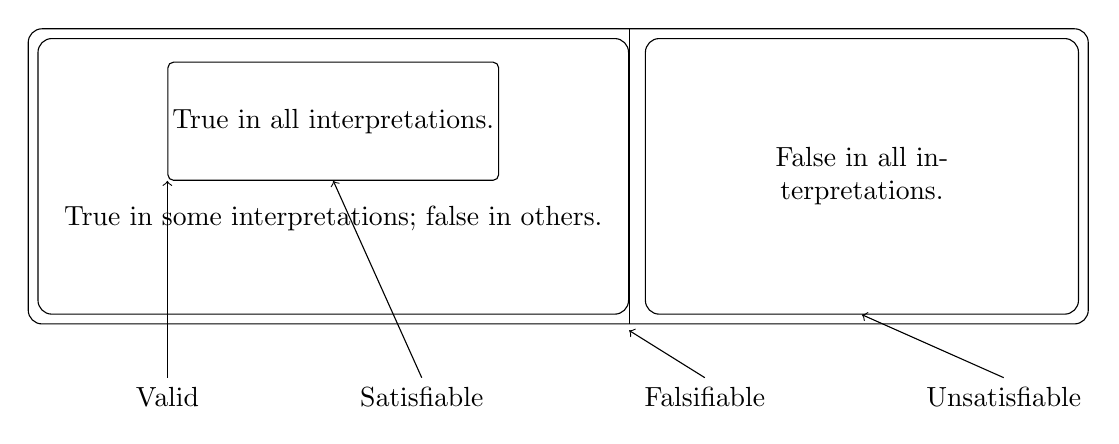
\begin{tikzpicture}
          % Define the two main regions first
          % Adjust minimum width/height and relative positioning for better fit
          \node (right_region) [draw, rounded corners=5pt, minimum width=5.5cm, minimum height=3.5cm, label={[text centered, text width=4cm]center:False in all interpretations.}] {};
          \node (left_region) [draw, rounded corners=5pt, minimum width=7.5cm, minimum height=3.5cm, left=0.2cm of right_region.west, anchor=east] {}; % Added label here
          \node [below=-1.5cm] at (left_region.south) {True in some interpretations; false in others.};
      
          % Draw the outer boundary using 'fit' to enclose the two regions
          \node (outer) [draw, rounded corners=5pt, fit=(left_region) (right_region)] {};
      
          % Inner node for "True in all interpretations"
          % Position it within the left region and adjust size
          \node (inner_true_all) [draw, rounded corners=2pt, minimum width=4.2cm, minimum height=1.5cm, below=0.3cm of left_region.north, anchor=north] {};
          \node [text centered] at (inner_true_all.center) {True in all interpretations.};
      
          % Add the vertical line between the two main regions, aligned with the outer box
          \draw (left_region.east |- outer.north) -- (left_region.east |- outer.south);
      
          % Labels at the bottom - adjust spacing
          \node (valid) [below=2.5cm of inner_true_all.south west] {Valid};
          \node (satisfiable) [right=1.8cm of valid.east] {Satisfiable};
          \node (falsifiable) [right=1.8cm of satisfiable.east] {Falsifiable};
          \node (unsatisfiable) [right=1.8cm of falsifiable.east] {Unsatisfiable};
      
          % Arrows - adjust start and end points
          \draw [->] (valid.north) -- (inner_true_all.south west);
          \draw [->] (satisfiable.north) -- (inner_true_all.south);
          \draw [->] (falsifiable.north) -- ([yshift=-0.2cm]left_region.south east); % Pointing slightly above the corner
          \draw [->] (unsatisfiable.north) -- (right_region.south);
      
        \end{tikzpicture}
      \end{latin}
      \renewcommand{\thefigure}{\lr{2.6}}
      \caption{Satisfiability and validity of formulas}
      \end{figure}

\subsection*{\lr{2.5.1} Decision Procedures in Propositional Logic}
    \begin{definition}[تعریف \lr{2.40}]
      فرض کنید $\mathscr{U} \subseteq \mathscr{F}$ مجموعه‌ای از فرمول‌ها باشد. الگوریتمی یک \emph{رویهٔ تصمیم} برای $\mathscr{U}$ است اگر برای هر فرمول دلخواه $A \in \mathscr{F}$ پایان یابد و پاسخ «بله» را بازگرداند اگر $A \in \mathscr{U}$ و پاسخ «خیر» را اگر $A \notin \mathscr{U}$.
      
      اگر $\mathscr{U}$ مجموعهٔ فرمول‌های قابل ارضا باشد، رویهٔ تصمیم برای $\mathscr{U}$ را \emph{رویهٔ تصمیم برای ارضاپذیری}\\ (\lr{decision procedure for satisfiability}) می‌نامیم\\ و به‌طور مشابه برای همگانی‌صادق‌بودن.
      
      با توجه به قضیهٔ \lr{2.39}، می‌توان از رویهٔ تصمیم برای ارضاپذیری به‌عنوان رویهٔ تصمیم برای همگانی‌صادق‌بودن استفاده کرد. برای تصمیم‌گیری دربارهٔ اینکه آیا فرمول $A$ همگانی‌صادق است یا نه، کافی است رویهٔ تصمیم برای ارضاپذیری را روی $\neg A$ اجرا کنیم. اگر گزارش دهد $\neg A$ قابل ارضا است، آنگاه $A$ همگانی‌صادق نیست؛ و اگر گزارش دهد $\neg A$ قابل ارضا نیست، آنگاه $A$ همگانی‌صادق است. چنین رویه‌ای را \emph{رویهٔ ابطال} \lr{(refutation procedure)} می‌نامند، زیرا به‌جای اثبات مستقیم اینکه فرمول همیشه درست است، تنها به جستجوی مثال نقض می‌پردازد که کارآمدی بیشتری دارد.
    \end{definition}
    
    وجود رویهٔ تصمیم برای ارضاپذیری در منطق گزاره‌ای بدیهی است، زیرا می‌توانیم برای هر فرمول یک جدول ارزش صدق بسازیم. جدول ارزش صدق در مثال \lr{2.21} نشان می‌دهد که $p \to q$ قابل ارضا ولی ناخودهمگانی‌صادق است؛ در مثال \lr{2.22} نشان داده شد که
    \[
    (p \to q) \;\leftrightarrow\; (\neg q \to \neg p)
    \]
    همگانی‌صادق است. مثال زیر یک فرمول ناتوان از ارضا را نمایش می‌دهد.
    
    \begin{example}[مثال \lr{2.41}]
      فرمول
      \[
      (p \lor q)\;\land\;\neg p\;\land\;\neg q
      \]
      ناتوان از ارضا است، زیرا در همهٔ سطرهای جدول ارزش صدق آن، مقدار \(F\) به‌دست می‌آید:
      
      \[
      \begin{array}{|c|c|c|c|c|c|}
      \hline
      p & q & p \lor q & \neg p & \neg q & (p \lor q)\land\neg p\land\neg q\\\hline
      $T$ & $T$ & $T$ & $F$ & $F$ & $F$\\
      $T$ & $F$ & $T$ & $F$ & $T$ & $F$\\
      $F$ & $T$ & $T$ & $T$ & $F$ & $F$\\
      $F$ & $F$ & $F$ & $T$ & $T$ & $F$\\\hline
      \end{array}
      \]
    \end{example}
    
    روش جدول ارزش صدق یک رویهٔ تصمیم بسیار ناکارآمد است؛ زیرا برای فرمولی با \(n\) اتم متمایز، باید آن را برای هر یک از \(2^n\) تعبیر ممکن ارزیابی کنیم. در فصول بعدی، رویه‌های تصمیم کارآمدتری برای ارضاپذیری ارائه خواهد شد، اگرچه بسیار بعید است رویهٔ تصمیمی وجود داشته باشد که برای همهٔ فرمول‌ها به‌طور کارآمد اجرا شود (به بخش \lr{6.7} مراجعه کنید).
\subsection*{\lr{2.5.2} ارضاپذیری یک مجموعه از فرمول‌ها}
    مفهوم \emph{ارضاپذیری} را می‌توان به \emph{مجموعه‌ای از فرمول‌ها} نیز تعمیم داد.
    
    \begin{definition}[تعریف \lr{2.42}]
    یک مجموعهٔ فرمول‌ها
    \[
    U = \{A_1, A_2, \dots\}
    \]
    هنگامی \emph{(به‌طور هم‌زمان) ارضاپذیر} است که تعبیری $\mathscr{I}$ وجود داشته باشد به‌گونه‌ای که برای همهٔ اندیس‌ها $i$ داشته باشیم:
    \[
    v_\mathscr{I}(A_i) = T.
    \]
    چنین تعبیری $\mathscr{I}$ را \emph{مدل} $U$ می‌نامیم.
    
    مجموعهٔ $U$ را \emph{ناتوان از ارضا} (unsatisfiable) می‌نامیم هرگاه برای \emph{هر} تعبیر $\mathscr{I}$، دست‌کم یک $i$ وجود داشته باشد که:
    \[
    v_\mathscr{I}(A_i) = F.
    \]
    \end{definition}
    
    \begin{example}[مثال \lr{2.43}]
    مجموعهٔ
    \[
    U_1 = \{p,\; \neg p \lor q,\; q \land r\}
    \]
    ارضاپذیر است، زیرا تعبیری که به هر سه اتم مقدار $T$ اختصاص دهد، همهٔ فرمول‌ها را ارضا می‌کند.
    
    اما مجموعهٔ
    \[
    U_2 = \{p,\; \neg p \lor q,\; \neg p\}
    \]
    ناتوان از ارضا است. هر فرمول از این مجموعه به‌تنهایی قابل ارضا است، ولی \emph{هم‌زمان با یکدیگر} ارضاپذیر نیستند.
    \end{example}
    
    اثبات قضایای ابتدایی زیر به‌عنوان تمرین باقی گذاشته شده‌اند:
    
    \begin{itemize}
      \item \textbf{قضیه \lr{2.44}}: اگر $U$ ارضاپذیر باشد، آنگاه برای هر $i$، مجموعهٔ
      \[
      U - \{A_i\}
      \]
      نیز ارضاپذیر است.
    
      \item \textbf{قضیه \lr{2.45}}: اگر $U$ ارضاپذیر باشد و $B$ فرمولی صادق همگانی (valid) باشد، آنگاه
      \[
      U \cup \{B\}
      \]
      نیز ارضاپذیر است.
    
      \item \textbf{قضیه \lr{2.46}}: اگر $U$ ناتوان از ارضا باشد، آنگاه برای هر فرمول $B$، مجموعهٔ
      \[
      U \cup \{B\}
      \]
      نیز ناتوان از ارضا است.
    
      \item \textbf{قضیه \lr{2.47}}: اگر $U$ ناتوان از ارضا باشد و برای بعضی $i$، فرمول $A_i$ صادق همگانی باشد، آنگاه
      \[
      U - \{A_i\}
      \]
      نیز ناتوان از ارضا خواهد بود.
    \end{itemize}
\subsection*{\lr{2.5.3} نتیجه‌ٔ منطقی \lr{(Logical Consequence)}}
    \begin{definition}[تعریف \lr{2.48}]
      فرض کنید $U$ مجموعه‌ای از فرمول‌ها و $A$ یک فرمول باشد. فرمول $A$ \textbf{نتیجه‌ٔ منطقی} $U$ است، اگر و تنها اگر هر \textbf{مدل} از $U$، مدل $A$ نیز باشد. این مفهوم با نماد
      \[
      U \models A
      \]
      نشان داده می‌شود.
      
      نیازی نیست که $A$ در \textbf{همهٔ تعبیرهای ممکن} صادق باشد، بلکه کافی است تنها در \textbf{تمام تعبیرهایی که $U$ را ارضا می‌کنند} (یعنی همهٔ فرمول‌های $U$ را درست می‌سازند) صادق باشد. اگر $U$ تهی باشد، نتیجه‌ٔ منطقی همان همگانی‌صادق بودن (validity) است.
    \end{definition}
    
    \begin{example}[مثال \lr{2.49}]
      بگذارید
      \[
      A = (p \lor r) \land (\neg q \lor \neg r).
      \]
      آنگاه
      \[
      \{p, \neg q\} \models A.
      \]
      زیرا $A$ در همهٔ تعبیرهایی که در آن‌ها $p =T$ و $q = F$ باشد، درست است. اما $A$ همگانی‌صادق نیست، زیرا در تعبیری مانند
      \[
      \mathscr{I}':\quad \mathscr{I}'(p) = F,\quad \mathscr{I}'(q) = T,\quad \mathscr{I}'(r) = T
      \]
      نادرست است.
    \end{example}
    
    نکته‌ای که پیش‌تر دربارهٔ تفاوت بین $\leftrightarrow$ و $\equiv$ گفته شد، دربارهٔ $\to$ و $\models$ نیز صدق می‌کند:
    
    \begin{itemize}
      \item $\to$ یک \textbf{عملگر} در زبان محتوایی منطق گزاره‌ای است،
      \item $\models$ یک \textbf{نماد مفهومی} در زبان مدرکی (ابردستگاه) است.
    \end{itemize}
    
    اما، همچون معادل منطقی، این دو مفهوم به‌هم مرتبط‌اند:
    
    \begin{theorem}[قضیه \lr{2.50}]
      اگر $U = \{A_1, A_2, \dots\}$، آنگاه:
      \[
      U \models A \quad \text{اگر و تنها اگر} \quad \models \left(\bigwedge_i A_i\right) \to A.
      \]
    \end{theorem}
    
    \begin{definition}[تعریف \lr{2.51}]
      عبارت
      \[
      \bigwedge_{i=1}^n A_i
      \]
      یعنی $A_1 \land A_2 \land \cdots \land A_n$. نماد $\bigwedge_i A_i$ هنگامی استفاده می‌شود که بازهٔ اندیس‌ها از متن قابل فهم باشد، یا اگر مجموعه فرمول‌ها نامتناهی باشد. برای جمع‌گزاره نیز از نماد مشابه $\bigvee_i A_i$ استفاده می‌شود.
    \end{definition}
    
    \begin{example}[مثال \lr{2.52}]
      از مثال \lr{2.49} داریم:
      \[
      \{p, \neg q\} \models (p \lor r) \land (\neg q \lor \neg r).
      \]
      پس طبق قضیه \lr{2.50}:
      \[
      \models (p \land \neg q) \to \bigl((p \lor r) \land (\neg q \lor \neg r)\bigr).
      \]
    \end{example}
    
    اثبات قضیهٔ \lr{2.50} و همچنین دو قضیهٔ زیر به‌عنوان تمرین باقی گذاشته شده‌اند:
    
    \begin{itemize}
      \item \textbf{قضیه \lr{2.53}.} اگر $U \models A$، آنگاه برای هر فرمول $B$،
      \[
      U \cup \{B\} \models A.
      \]
    
      \item \textbf{قضیه \lr{2.54}.} اگر $U \models A$ و فرمول $B$ همگانی‌صادق باشد، آنگاه
      \[
      U - \{B\} \models A.
      \]
    \end{itemize}
\subsection*{\lr{2.5.4} نظریه‌ها}
    نتیجهٔ منطقی، مفهوم مرکزی در بنیان‌های ریاضیات است.  
    فرمول‌های منطقی همواره‌صادق مانند
    \[
    p \lor q \leftrightarrow q \lor p
    \]
    اهمیت چندانی در ریاضیات ندارند. آنچه جالب‌تر است، \textbf{فرض گرفتن مجموعه‌ای از فرمول‌ها به‌عنوان صادق} و سپس \textbf{بررسی پیامدهای منطقی آن‌ها} است.
    
    برای مثال، اقلیدس پنج اصل دربارهٔ هندسه را فرض گرفت و مجموعهٔ گسترده‌ای از نتایج منطقی را از آن‌ها نتیجه گرفت.  
    تعریف صوری یک «نظریهٔ ریاضی» به‌صورت زیر است:
    
    \begin{definition}[تعریف \lr{2.55}]
      بگذارید $\mathscr{T}$ یک مجموعه از فرمول‌ها باشد. $T$ \textbf{تحت نتیجه‌ٔ منطقی بسته است} هرگاه برای هر فرمول $A$، اگر
      \[
        \mathscr{T} \models A,
      \]
      آنگاه
      \[
      A \in \mathscr{T}.
      \]
      مجموعه‌ای از فرمول‌ها که تحت نتیجه‌ٔ منطقی بسته باشد، یک \textbf{نظریه (theory)} نامیده می‌شود.  
      فرمول‌های عضو $\mathscr{T}$، \textbf{قضیه‌های (theorems)} نظریه نامیده می‌شوند.
    \end{definition}
    
    نظریه‌ها با انتخاب مجموعه‌ای از فرمول‌ها به‌عنوان \textbf{اصول موضوع (axioms)} ساخته می‌شوند و سپس \textbf{نتایج منطقی} آن اصول به نظریه افزوده می‌شوند.
    
    \begin{definition}[تعریف \lr{2.56}]
      اگر $\mathscr{T}$ یک نظریه باشد، آنگاه گفته می‌شود $\mathscr{T}$ \textbf{قابل اصل‌گذاری (axiomatizable)} است هرگاه \textbf{مجموعه‌ای از فرمول‌ها} مانند $U$ وجود داشته باشد به‌طوری‌که
      \[
      \mathscr{T} = \{A \mid U \models A\}.
      \]
      مجموعهٔ $U$ اصول موضوع نظریهٔ $\mathscr{T}$ هستند.  
      اگر $U$ متناهی باشد، آنگاه گفته می‌شود که $\mathscr{T}$ \textbf{قابل اصل‌گذاری به‌صورت متناهی} است.
    \end{definition}
    
    برای مثال، نظریهٔ حساب (\lr{Arithmetic}) قابل اصل‌گذاری است:  
    مجموعه‌ای از اصول توسط پئانو (\lr{Peano}) ارائه شده که نتایج منطقی آن‌ها، قضیه‌های حساب هستند.  
    اما نظریهٔ حساب \textbf{قابل اصل‌گذاری به‌صورت متناهی نیست}، چرا که اصل استقرا (\lr{induction axiom}) به‌صورت \textbf{یک طرح اصل} است که برای هر خاصیت در حساب، نمونه‌ای دارد و نمی‌توان آن را با تنها یک اصل بیان کرد.
\section*{\lr{2.6} جدول معنایی}

      روش جدول معنایی یک رویهٔ تصمیم‌گیری کارآمد برای بررسی ارضاپذیری (و به‌طور دوگانه، همگانی‌صدقی) در منطق گزاره‌ای است.  
      در فصل بعد، از جدول معنایی به‌طور گسترده برای اثبات قضایای مهم در مورد سیستم‌های استنتاجی استفاده خواهیم کرد.
      
      اصل بنیادین جدول معنایی بسیار ساده است:  
      با تجزیهٔ فرمول به مجموعه‌هایی از اتم‌ها و نقیض آن‌ها، در پی یافتن مدلی (تعبیری ارضاکننده) برای فرمول هستیم.
      
      بررسی امکان ارضا برای هر یک از این مجموعه‌ها آسان است:  
      یک مجموعه از اتم‌ها و نقیض اتم‌ها ارضاپذیر است اگر و تنها اگر شامل اتمی و نقیض همان اتم نباشد.  
      در نتیجه، فرمول اولیه ارضاپذیر است اگر حداقل یکی از این مجموعه‌ها ارضاپذیر باشد.
      
      اکنون با چند تعریف آغاز می‌کنیم و سپس ارضاپذیری دو فرمول را تحلیل می‌کنیم تا انگیزه‌ای برای ساختار جدول معنایی فراهم شود.

\subsection*{\lr{2.6.1} تجزیهٔ فرمول‌ها به مجموعه‌ای از لفظ‌ها}
  \begin{definition}[تعریف \lr{2.57}]
    یک \emph{لفظ} (literal)، یا \emph{اتم} است یا \emph{نفی یک اتم}.
    \begin{itemize}
      \item یک اتم، \emph{لفظِ مثبت} نامیده می‌شود.
      \item نفی یک اتم، \emph{لفظِ منفی} نام دارد.
    \end{itemize}
    برای هر اتم $p$، مجموعهٔ $\{p,\;\neg p\}$ یک \emph{زوج متمم} از لفظ‌ها تشکیل می‌دهد.  
    برای هر فرمول $A$، مجموعهٔ $\{A,\;\neg A\}$ نیز یک \emph{زوج متمم از فرمول‌ها} است.  
    فرمول $A$ متمم $\neg A$ و بالعکس است.
  \end{definition}
    
  \begin{example}[مثال \lr{2.58}]
    در مجموعهٔ لفظ‌ها
    \[
    \{\neg p,\; q,\; r,\; \neg r\}
    \]
    \begin{itemize}
      \item $q$ و $r$ لفظِ \emph{مثبت} هستند،
      \item $\neg p$ و $\neg r$ لفظِ \emph{منفی} هستند.
    \end{itemize}
    این مجموعه شامل زوج متمم $\{r,\neg r\}$ است.
  \end{example}
    
  \begin{example}[مثال \lr{2.59}]
    فرمول زیر را تحلیل می‌کنیم تا ارضاپذیری آن را در تعبیر دلخواه $\mathscr{I}$ بررسی کنیم:
    \[
    A = p \land (\neg q \lor \neg p).
    \]
    با استفاده از قواعد بازگشتی ارزیابی صدق:
    \begin{align*}
    v_{\mathscr{I}}(A)=T
    &\;\Longleftrightarrow\;
    v_{\mathscr{I}}(p)=T
    \;\land\;
    v_{\mathscr{I}}(\neg q\lor\neg p)=T,\\
    v_{\mathscr{I}}(\neg q\lor\neg p)=T
    &\;\Longleftrightarrow\;
    v_{\mathscr{I}}(\neg q)=T
    \;\lor\;
    v_{\mathscr{I}}(\neg p)=T.
    \end{align*}
    در نتیجه، $v_{\mathscr{I}}(A)=T$ اگر و تنها اگر یکی از دو حالت زیر برقرار باشد:
    \begin{enumerate}
      \item $v_{\mathscr{I}}(p)=T$ و $v_{\mathscr{I}}(\neg q)=T$
      \item $v_{\mathscr{I}}(p)=T$ و $v_{\mathscr{I}}(\neg p)=T$
    \end{enumerate}
    پس مسئلهٔ ارضاپذیری $A$ به بررسی ارضاپذیری دو مجموعهٔ لفظ‌ها کاهش می‌یابد.
  \end{example}
    
  \begin{theorem}[قضیه \lr{2.60}]
    مجموعه‌ای از لفظ‌ها \emph{ارضاپذیر} است \emph{اگر و تنها اگر} شامل هیچ \emph{زوج متممی} از لفظ‌ها نباشد.
  \end{theorem}
    
  \begin{proof}
    فرض کنید $L$ مجموعه‌ای از لفظ‌ها باشد که هیچ زوج متممی در آن وجود ندارد. تعبیر $\mathscr{I}$ را به‌صورت زیر تعریف می‌کنیم:
    \[
    \mathscr{I}(p)=
    \begin{cases}
    T, & \text{اگر  } p\in L,\\
    F, & \text{اگر  } \neg p\in L.
    \end{cases}
    \]
    این تعریف \emph{سازگار و کامل} است، زیرا در $L$ هیچ اتمی همراه نقیضش حضور ندارد. هر لفظِ موجود در $L$ در این تعبیر مقدار $T$ می‌گیرد؛ بنابراین $L$ ارضاپذیر است.
    
    حال اگر $\{p,\neg p\}\subseteq L$، در هر تعبیر ممکن یا $v_{\mathscr{I}}(p)=F$ یا $v_{\mathscr{I}}(\neg p)=F$ است، پس $L$ ارضاپذیر نخواهد بود.
  \end{proof}
    
  \begin{example}[مثال \lr{2.61}]
    ادامهٔ مثال \lr{2.59}:  
    برای $A = p\land(\neg q\lor\neg p)$، دو مجموعه‌ای که باید بررسی شوند:
    \[
    \{p,\neg p\}\quad\longrightarrow\quad\text{دارای زوج متمم}\;\to\;\text{ناتوان از ارضا},
    \]
    \[
    \{p,\neg q\}\quad\longrightarrow\quad\text{فاقد زوج متمم}\;\to\;\text{ارضاپذیر}.
    \]
    بنابراین فقط مجموعهٔ دوم ارضاپذیر است و از قضیهٔ \lr{2.60} تعبیری به‌دست می‌آید که در آن
    \[
    \mathscr{I}(p)=T,\quad \mathscr{I}(q)=F.
    \]
  \end{example}
    
  \begin{example}[مثال \lr{2.62}]
    اگر فرمول \emph{ناتوان از ارضا} باشد، مثلاً:
    \[
    B = (p\lor q)\land(\neg p\land\neg q),
    \]
    آنگاه:
    \begin{enumerate}
      \item برای ارضا شدن $B$ باید
        $v_{\mathscr{I}}(p\lor q)=T$ و $v_{\mathscr{I}}(\neg p\land\neg q)=T$.
      \item تجزیهٔ ترکیب عطفی و ترکیب فصلی نشان می‌دهد که دو حالت ممکن به مجموعه‌های لفظ‌ها می‌انجامد:
        \[
        \{p,\neg p,\neg q\},\quad \{q,\neg p,\neg q\}.
        \]
      \item هر دو شامل زوج متمم‌اند؛ بنابراین ناتوان از ارضا هستند (قضیهٔ \lr{2.60}).
    \end{enumerate}
    نتیجه می‌گیریم که \emph{هیچ مدلی برای $B$ وجود ندارد}، یعنی
    \[
   \text{ناتوان از ارضا است.} B\
    \]
  \end{example}
  
  \begin{figure}[ht]
    \centering
    \begin{latin}
      \resizebox{0.35\textwidth}{!}{
      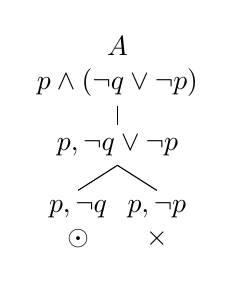
\begin{tikzpicture}[
        level distance=1cm,
        sibling distance=1.5cm,
        level 2/.style={sibling distance=1cm},
        edge from parent path={(\tikzparentnode.south) -- (\tikzchildnode.north)}
      ]
      \node[align=center] {$A$ \\ $p \land (\neg q \lor \neg p)$}
        child { 
          node {$p, \neg q \lor \neg p$}
          child { node[align=center] {$p, \neg q$ \\ $\odot$} }
          child { node[align=center] {$p, \neg p$ \\ $\times$} }
        };
      \end{tikzpicture}
      }
    \hfill
    \resizebox{0.35\textwidth}{!}{
      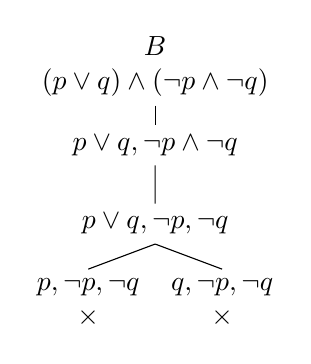
\begin{tikzpicture}[
        level distance=1cm,
        sibling distance=1.5cm,
        level 2/.style={sibling distance=1cm},
        level 3/.style={sibling distance=1.7cm},
        edge from parent path={(\tikzparentnode.south) -- (\tikzchildnode.north)}
      ]
      \node[align=center] {$B$ \\ $(p \lor q) \land (\neg p \land \neg q)$}
        child { 
          node {$p \lor q, \neg p \land \neg q$}
          child {
            node {$p \lor q, \neg p, \neg q$}
            child { node[align=center] {$p, \neg p, \neg q$ \\ $\times$} }
            child { node[align=center] {$q, \neg p, \neg q$ \\ $\times$} }
          }
        };
      \end{tikzpicture}
      }
    \end{latin}
    \renewcommand{\thefigure}{\lr{2.7}}
    \caption{درخت صدق}
  \end{figure}
\subsection*{\lr{2.6.2} ساخت جدول معنایی \lr{(Construction of Semantic Tableaux)}}
  
  تجزیهٔ فرمول به مجموعه‌ای از \emph{لفظ‌ها} در قالب متنی دشوار است. در روش \emph{جدول معنایی}، مجموعه‌های فرمول برچسبِ گره‌های یک درخت را تشکیل می‌دهند، به‌طوری که هر مسیر در درخت نمایانگر فرمول‌هایی است که باید در یک تعبیر ممکن صدق‌پذیر شوند.
  
  \begin{itemize}
    \item فرمول اولیه برچسبِ ریشهٔ درخت است.
    \item هر گره، بسته به نوع فرمول برچسب‌خورده، یک یا دو فرزند دارد.
    \item برگ‌ها با مجموعه‌ای از \emph{لفظ‌ها} برچسب می‌خورند.
    \item برگ‌هایی که شامل یک \emph{زوج متمم از لفظ‌ها} باشند با «$\times$» (بسته) و برگ‌هایی که فاقد زوج متمم هستند با $\odot$ (باز) علامت‌گذاری می‌شوند.
  \end{itemize}
  
  شکل \lr{2.7} جدول‌های معنایی مثال‌های پیشین را نشان می‌دهد. جدول زیر نمونهٔ دیگری از جدول معنایی برای فرمول
  \[
  B = (p \lor q)\;\land\;(\neg p \land \neg q)
  \]
  را نمایش می‌دهد که ابتدا برای $p \lor q$ منشعب شده و سپس $\neg p \land \neg q$ را پردازش می‌کند. واضح است که اگر \emph{همگرایی} ($\land$) را پیش از \emph{جمع‌گزاره} ($\lor$) بگشاییم، تعداد گره‌ها کمتر خواهد بود و در نتیجه کارآمدتر است.
  
  \begin{figure}[ht]
    \centering
    \begin{latin}
      \resizebox{0.35\textwidth}{!}{
      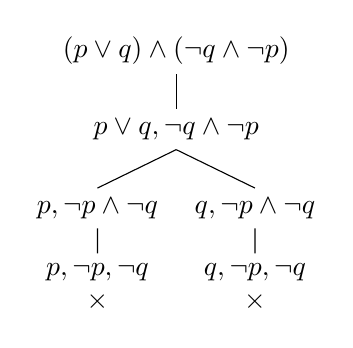
\begin{tikzpicture}[
        level distance=1cm,
        sibling distance=1.5cm,
        level 2/.style={sibling distance=2cm},
        level 2/.style={sibling distance=2cm},
        edge from parent path={(\tikzparentnode.south) -- (\tikzchildnode.north)}
      ]
      \node {$(p \lor q) \land (\neg q \land \neg p)$}
        child { 
          node {$p \lor q, \neg q \land \neg p$}
          child { 
            node {$p, \neg p \land \neg q$}
            child { node[align=center] {$p, \neg p, \neg q$ \\ $\times$} }
          }
          child { 
            node {$q, \neg p \land \neg q$}
            child { node[align=center] {$q, \neg p, \neg q$ \\ $\times$} }
          }
        };
      \end{tikzpicture}
      }
    \end{latin}
  \end{figure}
  
  برای ساده‌سازی و ایجاز، فرمول‌ها را بر اساس \emph{اپراتور اصلی} شان به دو دستهٔ \emph{$\alpha$-فرمول} و \emph{$\beta$-فرمول} تقسیم می‌کنیم (شکل \lr{2.8}):
  
  \begin{figure}[ht]
  \centering
  \begin{tabular}{|c|c|c|}
  \hline
  نوع & شکل عام & زیرفرمول‌ها \\
  \hline
  $\alpha$ & $A_1 \land A_2$ & $\alpha_1 = A_1,\;\alpha_2 = A_2$ \\
  $\alpha$ & $\neg(\neg A_1)$ & $\alpha_1 = A_1$ \\
  $\alpha$ & $\neg(A_1 \lor A_2)$ & $\alpha_1 = \neg A_1,\;\alpha_2 = \neg A_2$ \\
  $\alpha$ & $\neg(A_1 \to A_2)$ & $\alpha_1 = A_1,\;\alpha_2 = \neg A_2$ \\
  \hline
  $\beta$ & $A_1 \lor A_2$ & $\beta_1 = A_1,\;\beta_2 = A_2$ \\
  $\beta$ & $A_1 \to A_2$ & $\beta_1 = \neg A_1,\;\beta_2 = A_2$ \\
  $\beta$ & $\neg(A_1 \land A_2)$ & $\beta_1 = \neg A_1,\;\beta_2 = \neg A_2$ \\
  \hline
  \end{tabular}
  \renewcommand{\thefigure}{\lr{2.8}}
  \caption{طبقه‌بندی فرمول‌های آلفا و بتا}
  \end{figure}
  
  برای مثال، $p \land q$ یک $\alpha$-فرمول است (زیرا هر دو $p$ و $q$ باید صدق کنند)، و $\neg(p \land q)$ یک $\beta$-فرمول است (معادل $\neg p \lor \neg q$).
  
  \paragraph{\lr{2.64} الگوریتم ساخت جدول معنایی}
  \begin{enumerate}[1.]
    \item \textbf{ابتدایی‌سازی:}\\
      درختی با یک گرهٔ ریشه برچسب‌خورده $\phi$ بسازید. این گره هنوز علامت ندارد.
    \item \textbf{گسترش:}\\
      تا زمانی که برگ علامت‌نگرفته‌ای باقی بماند، مراحل زیر را تکرار کنید:
      \begin{enumerate}[a)]
        \item برگ $l$ را انتخاب کنید با مجموعهٔ برچسب $U(l)$ که هنوز علامت ندارد.
        \item اگر $U(l)$ \emph{مجموعه‌ای از لفظ‌ها} باشد:
          \begin{itemize}
            \item اگر شامل زوج متمم باشد، برگ را \emph{بسته} ($\times$) علامت بزنید.
            \item وگرنه، برگ را \emph{باز} ($\odot$) علامت بزنید.
          \end{itemize}
        \item در غیر این صورت (یعنی $U(l)$ شامل فرمول غیرلفظی است):
          \begin{enumerate}[(i]
            \item فرمولی $A\in U(l)$ را انتخاب کنید که \emph{لفظ} نباشد.
            \item بر اساس $\alpha$ یا $\beta$ بودن $A$ عمل کنید:
              \begin{itemize}
                \item \textbf{$\alpha$-فرمول:}\\
                  یک فرزند $l'$ بسازید با
                  \[
                  U(l') = \bigl(U(l) - \{A\}\bigr)\cup\{A_1,A_2\}.
                  \]
                  (اگر $A=\neg\neg A_1$ بود، تنها $\alpha_1$ را اضافه کنید.)
                \item \textbf{$\beta$-فرمول:}\\
                  دو فرزند $l'$ و $l''$ بسازید با
                  \[
                  U(l') = \bigl(U(l) - \{B\}\bigr)\cup\{B_1\},\quad
                  U(l'') = \bigl(U(l) - \{B\}\bigr)\cup\{B_2\}.
                  \]
              \end{itemize}
          \end{enumerate}
      \end{enumerate}
    \item \textbf{پایان:}\\
      وقتی هیچ برگ علامت‌نگرفته‌ای باقی نماند، الگوریتم تمام می‌شود.
  \end{enumerate}
  
  \begin{definition}[تعریف \lr{2.65}]
    \hfill
    \begin{itemize}
      \item جدولی که ساخت آن تکمیل شده، \emph{جدول تکمیل‌شده} نامیده می‌شود.
      \item یک جدول تکمیل‌شده \emph{بسته} است اگر \emph{همهٔ برگ‌ها} بسته ($\times$) باشند.
      \item در غیر این صورت (اگر دست‌کم یک برگ باز $\odot$ باشد)، جدول \emph{باز} است.
    \end{itemize}
  \end{definition}
 \subsection*{\lr{2.6.3} پایان‌پذیری ساخت جدول معنایی}

    از آنجا که هر گام از الگوریتم یک فرمول را به یک یا دو فرمول ساده‌تر فرو می‌شکند، بدیهی است که ساخت جدول معنایی برای هر فرمول خاتمه می‌یابد؛ با این حال، اثبات این ادعا ارزشمند است.
    
    \begin{theorem}[قضیه \lr{2.66}]
      ساخت جدول معنایی برای هر فرمول $\phi$ پایان‌پذیر است. هنگامی که ساخت خاتمه می‌یابد، تمام برگ‌ها با «$\times$» یا «$\odot$» علامت‌گذاری شده‌اند.
    \end{theorem}
    
    \begin{proof}
      فرض کنیم در فرمول $\phi$، عملگرهای $\leftrightarrow$ و $\oplus$ ظاهر نشوند (تعمیم به این دو مورد به‌صورت تمرین باقی گذاشته می‌شود).  
      برای هر برگ علامت‌نگرفته $l$ که در مرحله‌ای از گسترش انتخاب می‌شود، بگذارید
      \begin{align*}
      b(l) &\text{ تعداد کل عملگرهای دودویی موجود در همهٔ فرمول‌های }U(l),\\
      n(l) &\text{ تعداد کل نقیض‌ها در }U(l)
      \end{align*}
      سپس وزن
      \[
      W(l) \;=\; 3\,b(l) \;+\; n(l)
      \]
      را تعریف می‌کنیم.  
      برای مثال اگر
      \[
      U(l) = \{\,p \lor q,\;\neg p \land \neg q\},
      \]
      آنگاه $b(l)=2$ و $n(l)=2$ و بنابراین
      \[
      W(l) = 3\cdot 2 + 2 = 8.
      \]

      هر گام از الگوریتم یا یک گرهٔ جدید $l'$ یا دو گرهٔ جدید $l',l''$ را به‌عنوان فرزند $l$ می‌افزاید. ادعا می‌کنیم که در هر حالت:
      \[
      W(l') < W(l)
      \quad\text{و اگر گرهٔ دوم وجود داشته باشد،}\quad
      W(l'') < W(l).
      \]

      برای نمونه، فرض کنید فرمولی از نوع $\alpha$ داشته باشیم:
      \[
      A = \neg\,(A_1 \lor A_2),
      \]
      و قاعدهٔ $\alpha$ را روی برگ $l$ اعمال کنیم تا برگ جدید $l'$ برچسب‌خورد:
      \[
      U(l') = \bigl(U(l)\setminus\{\neg(A_1\lor A_2)\}\bigr)
      \;\cup\;\{\neg A_1,\;\neg A_2\}.
      \]
      در این صورت یکی از عملگرهای دودویی (یعنی $\lor$) و یک نقیض (علامت نفی بیرونی) حذف می‌شوند و دو نقیض جدید (برای $A_1$ و $A_2$) افزوده می‌شود. بنابراین:
      \[
      W(l') = W(l) - \bigl(3\cdot 1 + 1\bigr) + 2
      = W(l) - 2 < W(l).
      \]
      به همین ترتیب برای هر قاعدهٔ $\alpha$ یا $\beta$، وزن کاهش می‌یابد. از آنجا که $W(l)$ عددی طبیعی است و در هر گام کاهش پیدا می‌کند، الگوریتم نمی‌تواند بی‌پایان ادامه یابد و نهایتاً به برگ‌هایی منتهی می‌شود که همهٔ آن‌ها علامت‌گذاری شده‌اند.
    \end{proof}

\subsection*{\lr{2.6.4} بهبود کارایی الگوریتم}
  الگوریتم ساخت جدول معنایی «قطعی» نیست: در اکثر مراحل، انتخاب برگ برای گسترش و در صورتی که برگ بیش از یک فرمول غیرلفظی داشته باشد، انتخاب فرمول برای تجزیه آزاد است. این امکان را فراهم می‌کند که از \emph{هدایت‌کننده‌ها} (heuristics) استفاده کنیم تا جدول سریع‌تر تکمیل شود. همان‌طور که در بخش \lr{2.6.2} دیدیم، بهتر است ابتدا \emph{$\alpha$-فرمول‌ها} را باز کنیم و سپس \emph{$\beta$-فرمول‌ها} تا از تکرار بیهوده جلوگیری گردد.
  
  \paragraph{کوتاه‌سازی جدول با بستن زودهنگام شاخه: }
  می‌توان یک شاخه را به‌محض آنکه شامل یک فرمول و متمم آن شود (نه صرفاً یک زوج متمم از لفظ‌ها) بست. واضح است که ادامهٔ گسترش گره‌ای که برچسب
  \[
  \{\,p \land (q \lor r),\;\neg\bigl(p \land (q \lor r)\bigr)\}
  \]
  را دارد بی‌معنی است. اثبات اینکه این تغییر در صحت الگوریتم خللی ایجاد نمی‌کند به‌عنوان تمرین باقی گذاشته شده است.
  
  \paragraph{کاهش تکرارِ بازنویسی فرمول‌ها: }
  انتقال مکرر فرمول‌ها از یک گره به گرهٔ فرزند:
  \[
  U(l') = \bigl(U(l)\setminus\{A\}\bigr)\;\cup\;\{A_1,A_2\}
  \]
  منجر به تکرارهای بیهوده می‌شود. در گونه‌ای از جدول معنایی به نام \emph{جدول‌های تحلیلی}، هنگامی که گرهٔ جدیدی ایجاد می‌شود، تنها با \emph{فرمول‌های تازه} برچسب می‌خورد:
  \[
  U(l') = \{A_1, A_2\}.
  \]
  الگوریتم چنان تغییر می‌کند که فرمولی برای تجزیه انتخاب شود که در مسیر از ریشه تا برگ وجود دارد (به شرطی که تاکنون انتخاب نشده باشد).
  
  \begin{itemize}
    \item برگ «بسته» می‌شود اگر دو لفظ متمم (یا دو فرمول متمم) در برچسب‌های \emph{یک یا دو گره} در همان شاخه ظاهر شوند.
    \item برگ «باز» علامت می‌خورد اگر شاخه بسته نباشد و دیگر فرمولی برای تجزیه نمانده باشد.
  \end{itemize}
  
  \begin{example}
  برای فرمول
  \[
  B = (p \lor q) \land (\neg p \land \neg q)
  \]
  جدول تحلیلی به‌صورت زیر است؛ دقت کنید که پس از باز کردن $p \land q$، $p \lor q$ از گرهٔ دوم به گرهٔ سوم منتقل نمی‌شود:
  \\
    \begin{center}
    \begin{latin}
      \resizebox{0.3\textwidth}{!}{
      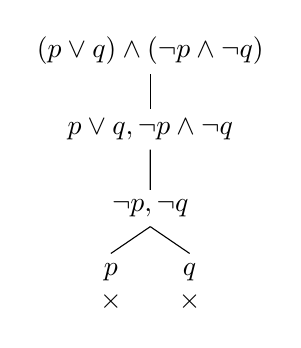
\begin{tikzpicture}[
        level distance=1cm,
        sibling distance=1.5cm,
        level 2/.style={sibling distance=1cm},
        edge from parent path={(\tikzparentnode.south) -- (\tikzchildnode.north)}
      ]
      \node {$(p \lor q) \land (\neg p \land \neg q)$}
        child { 
          node {$p \lor q, \neg p \land \neg q$}
          child { 
            node {$\neg p, \neg q$} 
            child { node[align=center] {$p$ \\ $\times$} }
            child { node[align=center] {$q$ \\ $\times$} }
          }
        };
      \end{tikzpicture}
      }  
    \end{latin}
    \end{center}
  با این حال، ما \emph{جدول معنایی کلاسیک} را ترجیح می‌دهیم زیرا در آن به‌وضوح دیده می‌شود که کدام فرمول‌ها نامزد تجزیه هستند و چگونه برگ‌ها علامت‌گذاری می‌گردند.
  
  \end{example}
\section*{\lr{2.7} صداپذیری و کاملیت \lr{(Soundness and Completeness)}}

    ساخت جدول معنایی یک فرایند کاملاً رسمی است. تجزیهٔ فرمول تنها مبتنی بر خواص نحوّی آن است: اپراتور اصلی فرمول و—در صورت منفی بودن—اپراتور اصلی فرمول منفی‌شده. تا کنون چند مثال برای انگیزهٔ جدول معنایی ارائه کردیم، اما صحت الگوریتم (ارتباط خروجی نحوی جدول با مفهوم معناشناختی ارزش صدق) را هنوز اثبات نکرده‌ایم. در این بخش نشان می‌دهیم که الگوریتم دقیقاً زمانی گزارش می‌دهد که فرمول ارضاپذیر یا ناتوان از ارضا است که مدل وجود دارد یا ندارد.
    
    روش‌های اثبات این بخش بسیار اهمیت دارد، زیرا در سیستم‌های منطقی دیگر بارها به‌کار گرفته می‌شوند.
    
    \begin{theorem}[قضیه \lr{2.67} صداپذیری و کاملیت]
      بگذارید $\mathscr{T}$ یک جدول تکمیل‌شده برای فرمول $A$ باشد. آنگاه:
      \[
      .\text{ ناتوان از ارضا است} A
      \;\Longleftrightarrow\;
      .\text{ بسته است} \mathscr{T}
      \]
    \end{theorem}
    
    از این قضیه چند نتیجهٔ مهم به‌دست می‌آید:
    
    \begin{corollary}[نتیجه‌گیری \lr{2.67}]
      فرمول $A$ ارضاپذیر است \emph{اگر و تنها اگر} $\mathscr{T}$ باز باشد.
    \end{corollary}
    
    \begin{proof}
      $A$ ارضاپذیر است $\iff$ (به‌تعریف) $A$ ناتوان از ارضا نیست  
      $\iff$ (با قضیهٔ \lr{2.67}) $\mathscr{T}$ بسته نیست  
      $\iff$ (به‌تعریف) $\mathscr{T}$ باز است.
    \end{proof}
    
    \begin{corollary}[نتیجه‌گیری \lr{2.68}]
      فرمول $A$ همگانی‌صادق (valid) است \emph{اگر و تنها اگر} جدول معنایی برای $\neg A$ بسته شود.
    \end{corollary}
    
    \begin{proof}
      $A$ همگانی‌صادق است  
      $\iff$ $\neg A$ ناتوان از ارضا است  
      $\iff$ جدول $\neg A$ بسته می‌شود.
    \end{proof}
    
    \begin{corollary}[نتیجه‌گیری \lr{2.70}]
      روش جدول معنایی یک رویهٔ تصمیم \lr{(decision procedure)} برای همگانی‌صدقی در منطق گزاره‌ای است.
    \end{corollary}
    
    \begin{proof}
      برای هر فرمول گزاره‌ای $A$، به کمک قضیهٔ \lr{2.66} ساخت جدول $\neg A$ پایان‌پذیر است و جدول تکمیل‌شده به‌دست می‌آید. از نتیجه‌گیری \lr{2.69} نتیجه می‌شود که  
      $A$ همگانی‌صادق $\iff$ جدول $\neg A$ بسته است.
    \end{proof}
    
    سمت مستقیم نتیجه‌گیری \lr{2.69} را \emph{کاملیت} (completeness) می‌نامند: اگر $A$ همگانی‌صادق باشد، با ساخت جدول برای $\neg A$ حتماً آن جدول بسته می‌شود.  
    جهت عکس را \emph{صداپذیری} (soundness) می‌گویند: هر فرمولی که جدول‌سازی آن را همگانی‌صادق اعلام کند (چون جدول $\neg A$ بسته است) واقعاً همگانی‌صادق است. در منطق، معمولاً اثبات صداپذیری آسان‌تر از اثبات کاملیت است؛ زیرا قواعد سیستم را طوری انتخاب می‌کنیم که آشکارا صداپذیر باشند، ولی سخت بتوانیم اطمینان یابیم که هیچ قاعدهٔ مفقودی نداریم که برای کاملیت ضروری باشد.
    
    به‌عنوان مثال، الگوریتم ضعیف زیر صداپذیر اما کاملاً ناقص است:
    
    \paragraph{الگوریتم \lr{2.71} \lr{(Incomplete decision procedure for validity)} \\}  
    \textbf{ورودی:} فرمول $A$ در منطق گزاره‌ای \\
    \textbf{خروجی:} گزارش «$A$ همگانی‌صادق نیست.»
    
    \begin{example}[مثال \lr{2.72}]
    اگر قاعدهٔ مربوط به $\neg(A_1 \lor A_2)$ را حذف کنیم، ساخت جدول هنوز صداپذیر خواهد بود، اما کاملیت را از دست می‌دهد. برای مثال فرمول واضحاً همگانی‌صادق
    \[
    A = \neg p \lor p
    \]
    را در نظر بگیرید. ریشهٔ جدول با $\neg A = \neg(\neg p \lor p)$ برچسب می‌خورد، اما هیچ قاعده‌ای برای تجزیهٔ این فرمول موجود نیست و بنابراین جدول بسته نمی‌شود، درحالی‌که $A$ به‌راستی همگانی‌صادق است.
    \end{example}

\subsection*{\lr{2.7.1} اثبات درستی}
  
  \begin{theorem}
  اگر جدول (tableau) \(\mathscr{T}\) برای فرمول \(A\) بسته شود، آنگاه \(A\) نارضایت‌پذیر \lr{unsatisfiable} است.
  \end{theorem}
  
  ما قضیه‌ای کلی‌تر را اثبات می‌کنیم:
  
  \begin{theorem}
  اگر زیر‌درخت \(\mathscr{T}_n\)، که در گرهٔ \(n\) از \(\mathscr{T}\) ریشه دارد، بسته باشد، آنگاه مجموعهٔ فرمول‌های \(U(n)\) که برچسب گرهٔ \(n\) است، نارضایت‌پذیر است.
  \end{theorem}
  
  درستیِ جدول (soundness) حالت خاصی از این قضیه است هنگامی که \(n\) همان گرهٔ ریشه باشد.
  
  برای سادگی اثبات، فرض می‌کنیم که فقط دو شکل از فرمول‌های \(\alpha\) و \(\beta\) داریم:
  \[
  \alpha\colon A_1 \land A_2,
  \qquad
  \beta\colon B_1 \lor B_2.
  \]
  
  \begin{proof}
  با استقرا بر ارتفاع \(h_n\) گرهٔ \(n\) در زیر‌درخت \(\mathscr{T}_n\).
  
  \textbf{قضیهٔ پایه} (\(h_n = 0\)).  
  اگر \(h_n=0\)، آنگاه \(n\) یک برگه (leaf) است و چون \(\mathscr{T}_n\) بسته است، در برچسب \(U(n)\) حتماً یک جفت متضاد از لیترال‌ها وجود دارد. بنابراین \(U(n)\) نارضایت‌پذیر است.
  
  \textbf{فرض استقرا}.  
  فرض کنید برای هر گرهٔ \(m\) با ارتفاع کمتر از \(h_n\) داریم:
  \[
  \forall m,\;h_m < h_n,\;\bigl[\mathscr{T}_m\ \text{بسته}\bigr]\;\Longrightarrow\;U(m)\ \text{نارضایت‌پذیر}.
  \]
  
  \textbf{گام استقرایی}.  
  حال گرهٔ \(n\) را در نظر بگیرید که \(h_n>0\). از آنجا که \(\mathscr{T}_n\) بسته است، حتماً روی \(n\) یکی از دو قاعدهٔ \(\alpha\) یا \(\beta\) اعمال شده است:
  \begin{center}
    \begin{latin}
      \resizebox{0.35\textwidth}{!}{
      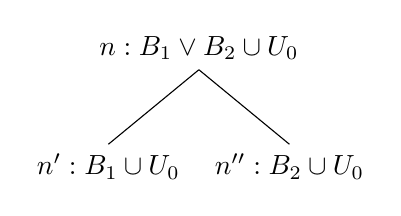
\begin{tikzpicture}[
        level distance=1.5cm,
        sibling distance=1.5cm,
        level 1/.style={sibling distance=2.3cm},
        edge from parent path={(\tikzparentnode.south) -- (\tikzchildnode.north)}
      ]
      \node {$n: {B_1 \lor B_2} \cup U_0$}
        child { 
          node {$n': {B_1} \cup U_0$}
        }
        child { 
          node {$n'': {B_2} \cup U_0$}
        };
      \end{tikzpicture}
      }  
    \hfill
    \resizebox{0.35\textwidth}{!}{
      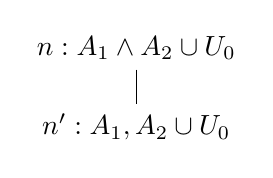
\begin{tikzpicture}[
        level distance=1cm,
        sibling distance=2.5cm,
        level 1/.style={sibling distance=2.5cm},
        level 2/.style={sibling distance=2.7cm},
        edge from parent path={(\tikzparentnode.south) -- (\tikzchildnode.north)}
      ]
      \node {$n: {A_1 \land A_2} \cup U_0$}
        child { node {$n': {A_1, A_2} \cup U_0$} };
      \end{tikzpicture}
      }
    \end{latin}
  \end{center}
  \begin{enumerate}[1)]
    \item \(\alpha\)\;  
      اگر قاعدهٔ \(\alpha\) (برای \(A_1\land A_2\)) روی \(n\) اعمال شده باشد، آنگاه
      \[
        U(n)=\{\,A_1\land A_2\}\cup U_0,
        \quad
        U(n')=\{\,A_1,\,A_2\}\cup U_0,
      \]
      و \(\mathscr{T}_{n'}\) نیز بسته است. از آنجا که ارتفاع \(n'\) برابر \(h_n-1\) است، به‌موجب فرض استقرا \(U(n')\) نارضایت‌پذیر است.  
      برای اثبات نارضایت‌پذیری \(U(n)\)، هر تفسیر دلخواه \(\mathscr{I}\) را در نظر بگیرید:
      \begin{itemize}
        \item اگر برای بعضی \(A_0\in U_0\)، \(v_{\mathscr{I}}(A_0)=F\)، چون \(U_0\subset U(n)\)، نتیجه می‌شود \(U(n)\) نارضایت‌پذیر است.
        \item در غیر این صورت \(v_{\mathscr{I}}(A_0)=T\) برای همهٔ \(A_0\in U_0\). چون \(U(n')\) نارضایت‌پذیر است، باید \(v_{\mathscr{I}}(A_1)=F\) یا \(v_{\mathscr{I}}(A_2)=F\).  
          اگر \(v_{\mathscr{I}}(A_1)=F\)، آنگاه
          \[
            v_{\mathscr{I}}(A_1\land A_2)=F,
          \]
          و چون \(A_1\land A_2\in U(n)\)، \(U(n)\) نارضایت‌پذیر است. (استدلال مشابه برای \(v_{\mathscr{I}}(A_2)=F\).)
      \end{itemize}
  
    \item \(\beta\)\;  
      اگر قاعدهٔ \(\beta\) (برای \(B_1\lor B_2\)) روی \(n\) اعمال شده باشد، آنگاه
      \[
        U(n)=\{\,B_1\lor B_2\}\cup U_0,\quad
        U(n')=\{\,B_1\}\cup U_0,\quad
        U(n'')=\{\,B_2\}\cup U_0,
      \]
      که هر دو \(\mathscr{T}_{n'}\) و \(\mathscr{T}_{n''}\) بسته‌اند و ارتفاع‌شان کمتر از \(h_n\) است. بنابراین \(U(n')\) و \(U(n'')\) نارضایت‌پذیرند.  
      برای هر تفسیر \(\mathscr{I}\):
      \begin{itemize}
        \item اگر برای بعضی \(B_0\in U_0\)، \(v_{\mathscr{I}}(B_0)=F\)، چون \(U_0\subset U(n)\)، آنگاه \(U(n)\) نارضایت‌پذیر است.
        \item وگرنه \(v_{\mathscr{I}}(B_0)=T\) برای همهٔ \(B_0\in U_0\).  
          از نارضایت‌پذیری \(U(n')\) و \(U(n'')\) داریم \(v_{\mathscr{I}}(B_1)=F\) و \(v_{\mathscr{I}}(B_2)=F\).  
          بنابراین
          \[
            v_{\mathscr{I}}(B_1\lor B_2)=F,
          \]
          و چون \(B_1\lor B_2\in U(n)\)، \(U(n)\) نارضایت‌پذیر است.
      \end{itemize}
  \end{enumerate}
  
  در هر دو حالت، نشان دادیم که اگر زیر‌درختهای فرزندان \(n\) بسته باشند، آنگاه \(U(n)\) نیز نارضایت‌پذیر است. این کامل‌کنندهٔ گام استقرایی است.
  
  بنابراین، به‌موجب اصل استقرا، برای هر گره \(n\)، اگر زیر‌درخت \(\mathscr{T}_n\) بسته باشد، آنگاه \(U(n)\) نارضایت‌پذیر است. حالت ویژه برای گرهٔ ریشه (\(n=\text{root}\)) اثبات می‌کند که اگر کل جدول \(\mathscr{T}\) بسته شود، آنگاه فرمول اولیه \(A\) نارضایت‌پذیر است.
  \end{proof}
\subsection*{\lr{2.7.2} اثبات کامل بودن \lr{(Completeness)}}
  
  \begin{theorem}
    اگر فرمول \(A\) نارضایت‌پذیر باشد، آنگاه هر جدولی (tableau) که برای \(A\) ساخته شود، بسته می‌شود.
  \end{theorem}
  
  برای اثبات، به‌جای مستقیم نشان می‌دهیم:
  
  \begin{corollary}[نتیجه گیری \lr{2.68}]
    اگر جدولی برای \(A\) باز باشد (یعنی دارای حداقل یک شاخهٔ باز)، آنگاه \(A\) برآورده‌پذیر (satisfiable) است.
  \end{corollary}
  
  روش کار در چهار گام اصلی است:
  \begin{enumerate}[1)]
    \item تعریف مجموعهٔ هینتیکا \lr{(Hintikka set)}.
    \item اثبات اینکه اجتماع برچسب‌های گره‌های یک شاخهٔ باز، یک مجموعهٔ هینتیکا است.
    \item اثبات اینکه هر مجموعهٔ هینتیکا برآورده‌پذیر است.
    \item نشان دادن اینکه خود فرمول \(A\) (برچسب ریشه) در آن مجموعه حضور دارد.
  \end{enumerate}
  
  \begin{definition}[مجموعهٔ هینتیکا]\label{def:2.75}
  مجموعه‌ای از فرمول‌ها را \emph{مجموعهٔ هینتیکا} می‌نامیم اگر:
  \begin{enumerate}[1)]
    \item برای هر اتم \(p\) که در مجموعه هست، دقیقاً یکی از \(p\in U\) یا \(\neg p\in U\) برقرار باشد.
    \item اگر \(A\in U\) یک فرمول \(\alpha\) باشد (یعنی \(A=A_1\land A_2\))، آنگاه \(A_1, A_2\in U\).
    \item اگر \(B\in U\) یک فرمول \(\beta\) باشد (یعنی \(B=B_1\lor B_2\))، آنگاه \(B_1\in U\) یا \(B_2\in U\).
  \end{enumerate}
  \end{definition}
  
  \begin{example}[مثال \lr{2.73}]
  فرض کنید
  \[
    A = p \land (\neg q \lor \neg p).
  \]
  یک جدول ممکن:
  \begin{center}
    \begin{latin}
      \resizebox{0.35\textwidth}{!}{
      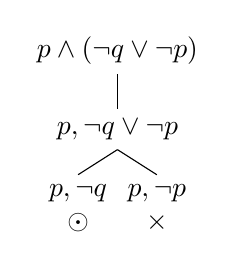
\begin{tikzpicture}[
        level distance=1cm,
        sibling distance=1.5cm,
        level 2/.style={sibling distance=1cm},
        edge from parent path={(\tikzparentnode.south) -- (\tikzchildnode.north)}
      ]
      \node {$p \land (\neg q \lor \neg p)$}
        child { 
          node {$p, \neg q \lor \neg p$}
          child { node[align=center] {$p, \neg q$ \\ $\odot$} }
          child { node[align=center] {$p, \neg p$ \\ $\times$} }
        };
      \end{tikzpicture}
      }  
    \end{latin}
  \end{center}
  شاخهٔ \(p,\neg q\) باز است با \(p=T,\,q=F\) که مدلی برای \(A\) می‌سازد.
  \end{example}
  
  \begin{example}[مثال \lr{2.74}]
  فرض کنید
  \[
    A = p \lor (q\land\neg q).
  \]
  یک جدول ممکن:
  \begin{center}
    \begin{latin}
      \resizebox{0.35\textwidth}{!}{
      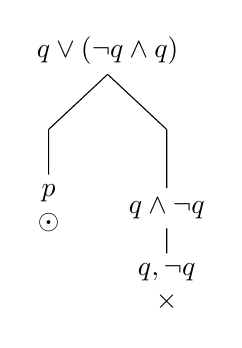
\begin{tikzpicture}[
        level distance=1cm,
        sibling distance=1.5cm,
        level 2/.style={sibling distance=1cm},
        edge from parent path={(\tikzparentnode.south) -- (\tikzchildnode.north)}
      ]
      \node {$q \lor (\neg q \land q)$}
        child { 
          child { node[align=center] {$p$ \\ $\odot$} }
        }
        child { 
          child { 
            node {$q \land \neg q$}
            child { node[align=center] {$q, \neg q$ \\ $\times$} }
          }
        };
      \end{tikzpicture}
      }  
    \end{latin}
  \end{center}
  شاخهٔ \(p\) باز است، پس هر مدلی باید \(p=T\) باشد.
  \end{example}
  
  \begin{theorem}[قضیهٔ \lr{2.77}]
  اگر \(l\) یک برگ باز در جدول تکمیل‌شده \(T\) باشد، آنگاه
  \[
    U \;=\;\bigcup_{i\in\text{شاخه از ریشه تا }l} U(i)
  \]
  یک مجموعهٔ هینتیکا است.
  \end{theorem}
  \begin{proof}
  \begin{enumerate}[1)]
    \item لیترال‌ها در هیچ قاعده‌ای شکسته نمی‌شوند و از ریشه تا برگ منتقل می‌گردند. چون برگ باز است، جفت متضاد در \(U(l)\) نیست، پس شرط (1) برقرار است.
    \item اگر \(A\in U\) یک \(\alpha\)-فرمول باشد، در مسیر تجزیه شده و زیرفرمول‌های \(A_1,A_2\) در \(U\) قرار می‌گیرند.
    \item اگر \(B\in U\) یک \(\beta\)-فرمول باشد، در مسیر تجزیه شده و یکی از زیرفرمول‌های \(B_1\) یا \(B_2\) در \(U\) قرار می‌گیرد.
  \end{enumerate}
  بنابراین \(U\) هینتیکا است.
  \end{proof}
  
  \begin{theorem}[لم هینتیکا \lr{2.78}]
  اگر \(U\) یک مجموعهٔ هینتیکا باشد، آنگاه \(U\) برآورده‌پذیر است.
  \end{theorem}
  \begin{proof}
  اتم‌های \(P_U\) را مجموعهٔ اتم‌های ظاهرشده در \(U\) در نظر بگیرید. تفسیر
  \(\mathscr{I}\) را تعریف می‌کنیم:
  \[
  \mathscr{I}(p)=
  \begin{cases}
  \mathsf{T}, & p\in U,\\
  \mathsf{F}, & \neg p\in U,\\
  \mathsf{T}, & \text{اگر }p,\neg p\notin U.
  \end{cases}
  \]
  شرط (1) تناقض را نفی می‌کند. سپس با استقرا بر ساختار فرمول‌ها نشان می‌دهیم برای هر \(A\in U\)، \(v_{\mathscr{I}}(A)=\mathsf{T}\):
  \begin{itemize}
    \item اگر \(A=p\) یا \(A=\neg p\)، واضح است.
    \item اگر \(A=A_1\land A_2\)، شرط (2) هر دو \(A_1,A_2\in U\) را تضمین می‌کند.
    \item اگر \(A=B_1\lor B_2\)، شرط (3) یکی از آنها را تضمین می‌کند.
  \end{itemize}
  پس \(\mathscr{I}\) مدلی از \(U\) است.
  \end{proof}
  
  \subsubsection*{نتیجه‌گیری}
  اگر \(T\) جدولی باز و تکمیل‌شده برای \(A\) باشد، اجتماع برچسب‌های شاخهٔ باز مجموعه‌ای هینتیکا می‌سازد (قضیهٔ \lr{2.77}) و از لم هینتیکا (قضیهٔ \lr{2.78}) این مجموعه مدل دارد. چون \(A\) در برچسب ریشه هست، \(\mathscr{I}\) مدلی برای \(A\) می‌شود و بنابراین اثبات کامل بودن پایان می‌یابد.

\end{document}